%\documentclass[serif,mathserif]{beamer}  % For use with beamer v 2.20
\documentclass[handout,serif,mathserif]{beamer}

%% NOTES %%%%%%%%%%%%%%%%%%%%%%%%%%%%%%%%%
\setbeameroption{hide notes} 

\usepackage{embedfile}
\IfFileExists{\jobname.nav}{\embedfile{\jobname.nav}}{}
% again, optional:
% just to keep things together
\embedfile{\jobname.tex}
%\embedfile{beamerthemeLausanne.sty}
%\embedfile{SplitShowIcon.png}
\newcommand{\emptynote}{\note{\mbox{}}}
%!TEX root = tutorial03-splitshow.tex
%!TEX root = tutorial03-slidesonly.tex



%%%%%%%%%%%%%%%%%%%%%%%%%%%%%%%%%%%%%%%%%%%%%%%%%%
%% IMPORTANT:
%% IN ORDER NOTES TO WORK WELL YOU HAVE TO ADD A NOTE TO EACH SLIDE!!!!
%% That is, at least a \emptynote command must be added to each slide.
%%%%%%%%%%%%%%%%%%%%%%%%%%%%%%%%%%%%%%%%%%%%%%%%%%

%\transdissolve

%	\setbeamercolor{postit}{fg=black,bg=yellow}
%	\begin{beamercolorbox}[sep=1em,wd=5cm]{postit}
%	Place me somewhere!
%	\end{beamercolorbox}


\usepackage{etex}
\usepackage[absolute,overlay]{textpos}
\usepackage{pdfsync, xspace}
\usepackage{pstricks,pst-node}
\usepackage{multimedia}
\usepackage[normal,tight,center]{subfigure}
\setlength{\subfigcapskip}{-.5em}
\usefonttheme[onlymath]{serif}

\mode<article> % only for the article version
{
  \usepackage{fullpage}
  \usepackage{hyperref}
}



\mode<presentation>
{
%  \setbeamertemplate{background canvas}[vertical shading][bottom=red!10,top=blue!10]
%  \setbeamertemplate{background canvas}
%  \usetheme{CambridgeUS}
  \usetheme{Boadilla}
}

%  There is a VERY rich set of possible
%  styles of presentations and color themes.  See the
%  beamer documentation for a full list of possibilities.
%\usetheme{Warsaw}  % JuanLesPins  Rochester
%\usetheme{JuanLesPins}

           %  Berkeley  Palo Alto    with sidebar and top
           % Goettingen  Marburg     with sidebar
           %  Copenhagen  Luebeck  Warsaw
%\usecolortheme{lily}
%\usecolortheme{default}
%\usecolortheme{crane}
\usecolortheme{beaver}


\usepackage{times}
\usepackage{multicol}
\setbeamercovered{dynamic}

%\usepackage{pgfarrows}
%  Don't need to load the pgf package, but it has
%  has itself some packages you might want, such as
%  pgfarrows,,pgfnodes,pgfautomata,pgfheaps
%  See the pgf documentation.


% \beamertemplatetransparentcovereddynamic
        % overlays that are upcoming are transparent, in
        % a manner that depends upon how far ahead  they are.


% \beamertemplatetransparentcovereddynamic
        % overlays that are upcoming are transparent, in
        % a manner that depends upon how far ahead  they are.

%\usepackage{beamerthemesplit}
%\usepackage{beamerthemebars}
% beamerthemelined
% beamerthemetree
% beamerthemetreebars
% Note: must be compiled with PDFLatex!!

%\usepackage{graphicx}
% support for Hungarian
%\usepackage[magyar]{babel}
%\usepackage[latin2]{inputenc}

%!TEX root = tutorial01-splitshow.tex


\usepackage[textwidth=\marginparwidth]{todonotes}
\usepackage{pdfsync}
\usepackage{hyperref}
\usepackage{fancybox}

% For citations
\newif\ifnumcites
%\numcitestrue
\numcitesfalse




% The paper has an extended (long) version and a short version
\newif\iflong % Sometimes we want to keep two versions; a short and a long one -- this is useful for that..
%\longfalse
\longtrue

% Turn on/off notes and descriptions of research problems
\newif\ifcomm
%\commfalse % also turns off internal todo comments
%\commtrue

% Turn on/off internal todo comments
\newif\iftodo
\todofalse
%\todotrue


\ifnumcites
  \usepackage[numbers]{natbib}
  \bibliographystyle{plainnat}
\else
  \usepackage{natbib}
  \bibliographystyle{apalike}
\fi
%\bibliographystyle{apalike}
% plain, acm, ieeetr, alpha, acm, abbrv, siam
% plainnat.bst, abbrvnat.bst and unsrtnat.bst
% http://web.reed.edu/cis/help/LaTeX/bibtexstyles.html

\if0
\newcommand{\citep}[1]{\cite{#1}}
\newcommand{\citet}[1]{\cite{#1}}
\newcommand{\citealt}[1]{\cite{#1}}
\newcommand{\iftextcite}[1]{}

\newcommand{\npcite}[1]{\cite{#1}}
\newcommand{\yrcite}[1]{\cite{#1}}
\fi



%\usepackage{amsthm}

\usepackage{amssymb}
%\usepackage[dvips]{graphics}
\usepackage{amsmath,amsthm,amsfonts} % Learn about the AMS package, again very useful!

\usepackage{graphicx}
\usepackage{epstopdf}
\usepackage{stmaryrd}
\usepackage{dsfont}
%\usepackage{small-headings}


\newif\ifshort
\iflong
	\shortfalse
\else
	\shorttrue
\fi


% THEOREMS -------------------------------------------------------
\theoremstyle{plain}
\newtheorem{thm}{Theorem}
\newtheorem{cor}[thm]{Corollary}
\newtheorem{lem}[thm]{Lemma}
\newtheorem{prop}[thm]{Proposition}
\newtheorem{conj}[thm]{Conjecture}
\newtheorem{proofthm}{Proof of Theorem 2}

%\renewtheorem{definition}[thm]{Definition}
\theoremstyle{definition}
\newtheorem{defn}{Definition}
%\theoremstyle{remark}


\newtheoremstyle{example}% ?name? 
{3pt}%	?Space above? 
{3pt}%	?Space below? 
{\itshape}%	?Body font?
{}%	?Indent amount?1 
{}% ?Theorem head font? 
{:}%	?Punctuation after theorem head? 
{.5em}%	?Space after theorem head?2 
{}%
\theoremstyle{example}
\newtheorem{ex}{Example}
%\newtheorem{fact}{Fact}
\newtheorem{rem}{Remark}

\newcounter{assumption}%[section]
\newcommand{\theassumptionletter}{A}
\renewcommand{\theassumption}{\theassumptionletter\arabic{assumption}}

\newenvironment{ass}[1][]{\begin{trivlist}\item[] \refstepcounter{assumption}%
 {\bf Assumption\ \theassumption\ #1} }{%\par\nobreak\noindent\sl\ignorespaces}{%
 \ifvmode\smallskip\fi\end{trivlist}}
\newcommand{\aref}[1]{(\ref{#1})}
\newenvironment{ass*}[1][]{\begin{trivlist}\item[] %
 {\bf Assumption\  #1} }{%\par\nobreak\noindent\sl\ignorespaces}{%
 \ifvmode\smallskip\fi\end{trivlist}}


%\newenvironment{remark}
\newtheorem{remark}{Remark}

%\newenvironment{proof}{{\bf Proof.}}{\hfill\rule{2mm}{2mm}\\}

% Keep whatever you need from here


\newcommand{\norm}[1]{\left\Vert#1\right\Vert}
\newcommand{\smallnorm}[1]{\|#1\|}
\newcommand{\abs}[1]{\left\vert#1\right\vert}
\newcommand{\supnorm}[1]{\norm{#1}_\infty}

\newcommand{\set}[1]{\left\{#1\right\}}
\newcommand{\cset}[2]{\left\{\,#1\,:\,#2\,\right\}}

\renewcommand{\natural}{\mathbb N}                   % Natural numbers
\newcommand{\Real}{\mathbb R}                        % Real numbers
\newcommand{\real}{\mathbb R}                        % again..
\newcommand{\R}{{\mathbb{R}}}                        % again..

\newcommand{\Prob}[1]{{\mathbb P}\left(#1\right)}    % Probabilities; example: \Prob{X>\eps}<1-\delta
\renewcommand{\P}{{\mathbb P}}                         % Probabilities when we want to control the parenthesis
\newcommand{\EE}[1]{{\mathbb E}\left[#1\right]}      % Expectations
\newcommand{\E}{{\mathbb E}}                         % Expectations  when we want to control the parenthesis
\newcommand{\Var}[1]{{\mathrm{Var}}\left[#1\right]}  % Variances
%\newcommand{\one}{\mathbb I}
\newcommand{\one}[1]{{\mathbb I}_{\{#1\}}}           % Characteristic function

\newcommand{\MB}{\mathcal{B}}
\newcommand{\MA}{\mathcal{A}}
\newcommand{\MS}{\mathcal{S}}
\newcommand{\MF}{\mathcal{F}}
\newcommand{\MC}{\mathcal{C}}
\newcommand{\MRR}{\mathcal{R}}
\newcommand{\MD}{\mathcal{D}}
\newcommand{\MP}{\mathcal{P}}
\newcommand{\MU}{\mathcal{U}}
\newcommand{\MO}{\mathcal{O}}
\newcommand{\MX}{\mathcal{X}}
\newcommand{\GG}{\mathcal{G}}
\newcommand{\hZ}{\hat{Z}}
\newcommand{\hF}{\hat{F}}
\newcommand{\hL}{\hat{L}}
\newcommand{\tL}{\tilde{L}}

\newcommand{\MI}{{\bf I}} %\mathbb{I}}


\newcommand{\eps}{\varepsilon}                       % Nice epsilon
\newcommand{\ep}{\varepsilon}                        % Shorthand for nice epsilon
\newcommand{\de}{\delta}                             % Shorthand for delta
\newcommand{\To}{\longrightarrow}
\newcommand{\ra}{\rightarrow}

\newcommand{\argmin}{\mathop{\rm argmin}}
\newcommand{\argmax}{\mathop{\rm argmax}}
\newcommand{\diag}{\mathop{\rm diag}}
\newcommand{\inlinemin}{\wedge}
\newcommand{\inlinemax}{\vee}

\newcommand{\ip}[2]{\langle #1,#2\rangle}
\newcommand{\bigip}[2]{\Big\langle #1,#2\Big\rangle}
\newcommand{\eqdef}{\stackrel{\mbox{\rm\tiny def}}{=}}
\newcommand{\aP}{{\cal P}}

% Shorthands I use for math environments
\newcommand{\beq}{\begin{equation}}
\newcommand{\eeq}{\end{equation}}
\newcommand{\beqa}{\begin{eqnarray}}
\newcommand{\eeqa}{\end{eqnarray}}
\newcommand{\beqan}{\begin{eqnarray*}}
\newcommand{\eeqan}{\end{eqnarray*}}
\newcommand{\ben}{\begin{eqnarray*}}
\newcommand{\een}{\end{eqnarray*}}

\newcommand{\RA}{$\Rightarrow$}

\newcommand{\TODO}[2][]{\todo[#1]{#2}}

\iflong
\else
	\renewcommand{\note}[2][]{}
	\renewcommand{\bibnote}[2][]{}
	\renewcommand{\problem}[2][]{}
\fi

\ifcomm
   \newcommand\comm[1]{\textcolor{blue}{ #1}}
\else
   \newcommand\comm[1]{}
%   \renewcommand{\todo}[1]{}
   \renewcommand{\todo}[2][]{}
\fi

\iftodo
\else
  \renewcommand{\TODO}[2][]{}
\fi

\newcommand{\remove}[1]{\textcolor{blue}{\sout{#1}}}
\newcommand{\tO}{\tilde{O}}

% Boldfaced lowercase greek letters as described at
% http://www.rpi.edu/dept/acs/rpinfo/common/Computing/Consulting/Software/LaTeX/Hints/Greek_Chars.html
\def\bmath#1{\mbox{\boldmath$#1$}}
% http://www.ctan.org/tex-archive/info/symbols/comprehensive/symbols-a4.pdf page 68
\newcommand\independent{\protect\mathpalette{\protect\independenT}{\perp}}
\def\independenT#1#2{\mathrel{\rlap{$#1#2$}\mkern2mu{#1#2}}}


\newcommand{\Set}{S}
\newcommand{\States}{\mathcal{X}}
\newcommand{\Actions}{\mathcal{A}}
\newcommand{\TranKernel}{\mathcal{P}}
\newcommand{\JTranKernel}{\mathcal{P}_{0}}
\newcommand{\PKernel}{\mathcal{P}}
\newcommand{\RKernel}{\mathcal{Q}}
\newcommand{\st}{x}
\newcommand{\St}{X}
\renewcommand{\action}{a}
\newcommand{\nextaction}{a'}
\newcommand{\Action}{A}
\newcommand{\Nextaction}{A'}
\newcommand{\reward}{r}
\newcommand{\Reward}{R}
\newcommand{\Ret}{\mathcal{R}}
\newcommand{\MDP}{\mathcal{M}}
\newcommand{\nextstate}{y}
\newcommand{\Nextstate}{Y}
\newcommand{\rewardfun}{r}
\newcommand{\TransPOp}{P}
\newcommand{\id}{I}

\renewcommand{\atop}{^{\top}}
\newcommand{\SA}{\States\times\Actions}


\newcommand{\astate}{z}
\newcommand{\AStates}{Z}%\State_A}
\newcommand{\APKernel}{\PKernel_A}
\newcommand{\rewardrange}{{\mathcal R}}
\iflong
\newcommand{\myfootnote}[1]{\footnote{#1}}
\else
\newcommand{\myfootnote}[1]{}
\fi
\renewcommand{\epsilon}{\varepsilon}

\newcommand{\tder}{\nabla_\theta}
\newcommand{\tders}{\nabla_\theta}
\newcommand{\pder}{\frac{\partial}{\partial \theta}}
\newcommand{\pders}{\tfrac{\partial}{\partial \theta}}


\newcommand{\pai}{{(i)}}
\newcommand{\integer}{\mathbb{Z}}
\newcommand{\cD}{{\cal D}}
\newcommand{\cZ}{{\cal Z}}
\newcommand{\cX}{{\cal X}}
\newcommand{\cW}{{\cal W}}

\newcommand{\cG}{{\cal G}}
\newcommand{\cF}{{\cal F}}
\newcommand{\cH}{{\cal H}}
\renewcommand{\phi}{\varphi}
\newcommand{\ewithin}{\eps_{\text{W}}}
\newcommand{\ebetween}{\eps_{\text{B}}}
\newcommand{\emean}{\eps_{\text{M}}}
\DeclareMathOperator{\trace}{trace}
\newcommand{\e}{\mathbf{1}}
\renewcommand{\eps}{\varepsilon}
\newcommand{\cM}{{\cal M}}
\newcommand{\cS}{{\cal S}}
\newcommand{\tM}{\tilde{M}}
\newcommand{\MRP}{{\cal M}}
\newcommand{\kfun}{\mathbb{K}}
\newcommand{\cK}{{\cal K}}

\newcommand{\aparam}{\omega}
\newcommand{\dimaction}{d_{\Actions}}
\newcommand{\dimaparam}{d_{\aparam}}
\newcommand{\traj}{\xi}
\newcommand{\Trajset}{\Xi}
\newcommand{\Traj}{X}
\newcommand{\perf}{\rho}
\newcommand{\dstat}{\mu} % stationary distribution underlying a Markov chain
\newcommand{\Regret}{{\bf R}}
\renewcommand{\AA}{{\cal A}}
%\newcommand{\SA}{\States\times\Actions}
\newcommand{\Sample}{{\cal D}}
\newcommand{\hA}{\hat{A}}
\newcommand{\hb}{\hat{b}}
\newcommand{\ZZ}{{\cal Z}}
\newcommand{\ttop}{^\top}
\newcommand{\FF}{{\cal F}}
\newcommand{\PiStat}{\Pi_{\rm stat}}
\newcommand{\td}{\delta}
\newcommand{\hV}{\hat{V}}
\newcommand{\mynote}[1]{}
\newcommand{\elg}{z}
\newcommand{\furtherreading}{}
\newcommand{\rfun}{\reward}
\newcommand{\pscorefun}[1]{\frac{\partial \ln \pi_\aparam(#1)}{\partial \aparam}}
\newcommand{\pscorefunp}[1]{\frac{\partial}{\partial\aparam}\,\log \pi_\aparam(#1)}
\newcommand{\scorefun}{\psi}
\newcommand{\hQ}{\hat{Q}}
\renewcommand{\th}{^{\rm th}}
\newcommand{\bee}{\begin{enumerate}}
\newcommand{\eee}{\end{enumerate}}

\usepackage{algorithm}
\usepackage{algpseudocode}
\algnewcommand\algorithmicto{\textbf{to}}
\algnewcommand\algorithmicdownto{\textbf{downto}}

%!TEX root = tutorial01-splitshow.tex

\usepackage{wasysym} % for \smiley \frownie
%
% \usepackage{wrapfig}
% \begin{wrapfigure}{POS}{WIDTH}{LINES TO RESERVE}
% ..
% \end{wrapfigure}
% The last argument is optional

% Figures need exact positioning in columns
% Use the following command to place them
\newcommand{\figincol}[1]{
\pgfputat{\pgfxy(0,0)}{\pgfbox[left,top]{#1}}
}

% ALSO:
% \pgfputat {\pgfxy(XX,YY)}{\pgfbox[left,base]{#1}}
% 
% LL = (0cm,-7cm) 
% UR = (11cm,1cm)
%
% pgfdeclareimage
% pgfuseimage

\newcommand{\Ra}{\Rightarrow}
%% BEAMER SPECIFIC COMMANDS

\newcommand{\bi}{\begin{itemize}}
\newcommand{\ei}{\end{itemize}}
\newcommand{\bc}{\begin{center}}
\newcommand{\ec}{\end{center}}


\setbeamercolor{math text}{fg=blue!50!normal text.fg}
\newcommand{\animframe}[2]{\begin{frame}[<+->]{#1}#2\end{frame}}
\newcommand{\animframesq}[2]{\begin{frame}[<+->][shrink,squeeze]{#1}#2\end{frame}}
\newcommand{\animframejsq}[2]{\begin{frame}[<+->][squeeze]{#1}#2\end{frame}}

\newcommand{\animframen}[2]{\begin{frame}[<+->]{#1}#2\emptynote\end{frame}}
\newcommand{\animframesqn}[2]{\begin{frame}[<+->][shrink,squeeze]{#1}#2\emptynote\end{frame}}
\newcommand{\animframejsqn}[2]{\begin{frame}[<+->][squeeze]{#1}#2\emptynote\end{frame}}

\newcommand{\myframe}[2]{\begin{frame}{#1}#2\end{frame}}
\newcommand{\myframesq}[2]{\begin{frame}[shrink,squeeze]{#1}#2\end{frame}}
\newcommand{\myframejsq}[2]{\begin{frame}[squeeze]{#1}#2\end{frame}}

\newcommand{\myframen}[2]{\begin{frame}{#1}#2\emptynote\end{frame}}
\newcommand{\myframesqn}[2]{\begin{frame}[shrink,squeeze]{#1}#2\emptynote\end{frame}}
\newcommand{\myframejsqn}[2]{\begin{frame}[squeeze]{#1}#2\emptynote\end{frame}}


%\setbeamertemplate{footline}[frame number]
\newtheorem{Solution}[theorem]{Solution}
\newtheorem{Comm}[theorem]{Comment}
\newtheorem{Note}[theorem]{Note}

\newcommand{\bcol}[1][t]{\begin{columns}[#1]} % optional argument: alignment (t,b,c)
\newcommand{\ecol}{\end{columns}}
\newcommand{\col}[1][0.5\textwidth]{\column{#1}} % argument: width of the column
%\parindent = 10pt
\newcommand{\scaletext}[3]{ % scale-factor original-width TEXT
\scalebox{#1}{\begin{minipage}[h]{#2\textwidth} #3 \end{minipage}
}}

% note: beamer slides are 128mm by 96 mm
\newcommand{\putatUL}[4]{ % width xpos ypos WHAT; upper left corner is put at the said pos
\begin{textblock*}{#1}[0,0](#2,#3)
#4
 \end{textblock*}
}
\newcommand{\putatBR}[4]{ % width xpos ypos WHAT; bottom right corner is put at the said pos
\begin{textblock*}{#1}[1,1](#2,#3)
#4
 \end{textblock*}
}
\newcommand{\putatBL}[4]{ % width xpos ypos WHAT; bottom left corner is put at the said pos
\begin{textblock*}{#1}[0,1](#2,#3)
#4
 \end{textblock*}
}
\newcommand{\putatUR}[4]{ % width xpos ypos WHAT; bottom right corner is put at the said pos
\begin{textblock*}{#1}[1,0](#2,#3)
#4
 \end{textblock*}
 }
 \newcommand{\putatMID}[4]{ % width xpos ypos WHAT; bottom right corner is put at the said pos
\begin{textblock*}{#1}[0.5,0.5](#2,#3)
#4
 \end{textblock*}
 }

\newcommand{\putat}[3]{\begin{picture}(0,0)(0,0)\put(#1,#2){#3}\end{picture}} % xrelpos yrelpos WHAT

\makeatletter
\newcommand{\insertprevframe}[1]{
	\def\beamer@origlmargin{\Gm@lmargin}
%    \vbox{\hfill\insertslideintonotes{0.125}\hskip-\Gm@rmargin\hskip0pt%
%      \vskip-0.125\paperheight\nointerlineskip}%
	\insertslideintonotes{#1}
}

%\newcommand{\insertslideintonotes}[1]{{%
%  \begin{pgfpicture}{0cm}{0cm}{#1\paperwidth}{#1\paperheight}
%    \begin{pgflowlevelscope}{\pgftransformscale{#1}}%
%      \color[gray]{0.8}
%      \pgfpathrectangle{\pgfpointorigin}{\pgfpoint{\paperwidth}{\paperheight}}
%      \pgfusepath{fill}
%      \color{black}
%      {\pgftransformshift{\pgfpoint{\beamer@origlmargin}{\footheight}}\pgftext[left,bottom]{\copy\beamer@frameboxcopy}}
%    \end{pgflowlevelscope}
%  \end{pgfpicture}%
%  }}
\makeatother
% For adding items to the notes pages (we do not want animation there)
\newcommand{\bin}{\bi[<1->]}


\title[RL Algorithms]{
Reinforcement Learning Algorithms in Markov Decision Processes\\
AAAI-10 Tutorial\\
\mbox{}\\
Part III: Learning to control
}
\author[Szepesv\'ari \& Sutton]{Csaba Szepesv\'ari \and Richard S. Sutton}
\institute[UofA]{
University of Alberta\\
E-mails: {\bf \{szepesva,rsutton\}@.ualberta.ca}\\
}
\date[July 11, 2010]{Atlanta, July 11, 2010}

\begin{document}

\frame{
	\titlepage
	\putatBL{10mm}{10mm}{66mm}{\includegraphics<+->[width=10mm]{Figures/Szepesvari.jpg}}
	\putatBR{10mm}{118mm}{66mm}{\includegraphics<.->[width=10mm]{Figures/Sutton}}
	% 128 x 96 mm
	\putatMID{20mm}{64mm}{85.5mm}{
	
\includegraphics[width=10mm]{Figures/rlai}
	
\includegraphics[width=10mm]{Figures/UofA-lowRes}
	}
	\emptynote
}

%\maketitle
\section<presentation>*{Outline}

\begin{frame}
  \frametitle{Outline}
  %\scriptsize
  \tableofcontents[part=1] %,pausesections]
    \emptynote

\end{frame}

\AtBeginSubsection[]
{
  \begin{frame}<beamer>
    \frametitle{Outline}
    \tableofcontents[current,currentsubsection]
    \emptynote
  \end{frame}
}

\part<presentation>{Main Talk}

\section{Introduction}
\animframesqn{The landscape}
{
\bc
\includegraphics<+->[width=0.8\textwidth]{Figures/learning-scenarios}
\ec
\note{
\bin \small
\item 
First criterion: can the learner actively  influence the observations?
\bin
\item YES:  {\em interactive learning}, NO: {\em non-interactive learning}
\item[] ``active learning''/ ``passive learning'' would work, but they are overloaded.
\ei
\item Interactive learning: potentially easier (since the learner has the additional option to influence the distribution of the sample).
\item However, the goals are usually different!!! INCOMPARABLE SITUATIONS!
\item Non-interactive learning: e.g., ``batch learning'' (learning given some data pool)
\item Interactive learning:
\bin
\item Online learning: goal is to maximize reward while learning; ``regret'' is the cost of learning
\item Active learning: goal is to find a good policy quickly ($\approx$ experimental design)
\ei
\ei
}
}

\section{Closed-loop, interactive learning}

\animframen{Bandit problems: \small How to gamble if you must? Part II}
{
\begin{block}{Bandit problem}
\bi
\item MDP with single state
\item Unknown distribution of rewards
\item Which action to choose so as to minimize the regret,
\[
L_T = T \max_{\action\in\Actions} \rewardfun(\action)  \,\, - \sum_{t=1}^T \Reward_t.
\]
\vspace*{-0.2in}
\ei
\end{block}
\bi
\item \citet{LaiRo85}: \alert{optimism in the face of uncertainty} (OFU) principle:
\begin{quote}
Choose the action with the best potential where  the uncertainty of the available information is taken into account
\end{quote}
\item They ``solved'' the parametric case: $\log$ regret, matching upper and lower bounds
\ei
}
\animframesqn{Bandit problems: Nonparametrics}
{
\bi
\item \citet{AuerBandit}: When the distributions can be arbitrary ($\Reward_t\in [0, \rewardrange]$), play the action maximizing
\[
U_t(\action) = \reward_t(\action) + \rewardrange\, \sqrt{\frac{2 \log t}{n_t(\action)}}.
\]
\item Upper Confidence Bound: UCB $\Rightarrow$ UCB1 algorithm
\item Main result: $L_T = O(\log(T))$
\item The minimax regret is $O(\sqrt{T})$.
\item By estimating the variance the expected regret can be improved, but there is a bias-variance tradeoff % \citet{AuMuSze09}
\ei
\note{
\bin
\item $\reward_t(\action)$ is the empirical estimate of the reward of action $a$ based on $n_t(\action)$ samples
\item The bound is not far from the best possible
\item UCB1 is indeed a good, proven algorithm
\item Other heuristic approaches:
\bin
\item $\epsilon$-greedy, $\epsilon_t =c/t$, $c$ must be chosen in a problem dependent manner
\item Boltzmann exploration (works in the adversarial bandit setting!)
\ei
\ei
}
}

\animframe{Beware the risk!}
{
\bc
\includegraphics<+->[width=\textwidth]{Figures/UCB-V-Regret}

Distribution of the regret for UCB-V at times $T_1 = 16,384$ (l.h.s. figure) and $T_2 = 524,288$ (r.h.s. figure)
on a two-armed bandit, where the payoff of the optimal arm is Ber($0.5$), and the payoff of the suboptimal arm is $0.495$.

\ec
\note{
	This is a side story, that can be left out.
	
	We often concentrate on the expected performance, like the expected reward.
	We like to argue that, by the law of large numbers or the central limit theorem, it suffices to optimize so that we maximize the expected reward.
	
	However, one has to be careful, since in some cases the distribution of the cumulated reward (or regret) may take funny shapes
	and then the expected performance may not be a good representative of the performance.
	
	The example shows the behavior of UCB-V, which is just like UCB1, but the variance is estimated on-line and is used in the action
	selection with an appropriate correction term. The performance of UCB-V, in terms of expected regret, is superior to that of UCB1.
	Yet, its risk can be higher.
	
}
}

\animframesqn{Online learning: Epilogue}
{
\bi
\item Bayesian bandits
\bi
\item The issue is not conceptual, but computational
\item \citet{gittins89}: ``Gittins index'' (cheap computation)
\item The Bayesian setting applies e.g. in poker (we know the distribution of cards)
\ei
\item Active learning in bandits
\bi
\item ``Action elimination''
\item These algorithms are unimprovable  \citep{EvenDarMM2002,TsiMa04,MniSzeAu08}.
\ei
\item Online learning in MDPs
\bi
\item UCRL2 by  \citet{AuJaOr10} implements the OFU principle
\item Individual rate: $O(\log T)$, minimax: $O(\sqrt{T})$
\ei
\item PAC-MDP algorithms
\bi
\item ``Mistake bounds''
\item R-MAX, MBIE, OI, {\sc MorMax}, Delayed-Q, ..
\item \citep{kearnssingh:icml98,BraTen02,KakadeThesis:2003,StrehlLittman2005,StrLiWieLaLi08,SziLo08,SziSze10}
\ei
\ei
\note{
\bin
\item UCRL2 bounds:
{\tiny
\bin 
\item w.p. $1-3\delta$,
$
\Regret_T^{\mathrm{UCRL2}(\delta)}  = O(D^2 |\States|^2 |\Actions|\log (T/\delta)/\eps + \eps T),
$
where $D$, the so-called {\em diameter} of the MDP
\item {\tiny 
  the largest number of steps (on average) it takes to reach some state from some other state
  in the MDP}
\item $\EE{\Regret_T^{\mathrm{UCRL2}(1/(3T))}} = O(D^2 |\States|^2 |\Actions|\log(T)/g)$,
 where $g$ is the ``gap'' between the performance of the optimal policy and the second best policy
\item Minimax bound:
$\EE{\Regret_T^{\mathrm{UCRL2}(1/(3T))}} = O(D  |\States| \sqrt{ |\Actions| T \log T }).$
\ei
}
\item {\sc MorMax} bound:
	  \[
	  T_\eps=\tilde{O}\left(
	  	 |\States|\,|\Actions| \left(\frac{V_{\max}}{\eps(1-\gamma)^2}\right)^2 \log\left(\frac{1}{\delta}\right)
	  	 \right).
	  \]
\item Theory nice, however, at the moment scaling is a problem
\item Current research: understand the situation for bandits with infinitely many arms
\item Practice: $\epsilon$-greedy, Boltzmann, \alert{optimistic initialization}
\ei
}
}

\section{$Q$-learning -- a direct method}

\animframejsqn{Goal}
{
\begin{alertblock}{Idea/Goal}
\bigskip
\bigskip
\bc
Learn $Q^*$ directly.
\ec
\bigskip
\end{alertblock}
\note{
\vspace*{-0.1in}
\bi
\item Remember the ``Fundamental Theorem''
\item The idea is that the knowledge of $Q^*$ alone is sufficient to know how to act optimally!
\bin
\item At least, when $\argmax_{\action\in\Actions} Q^*(\st,\action)$ can be computed easily
\item This is problematic when the number of actions is large, unless $Q^*(\st,\cdot)$ assumes some easily optimizable form
\ei
\item Sometimes {\tiny (games, resource management, etc.)} one may use \alert{post-decision state value function} $V_A$. 
\item Assumption:
$
\st  \stackrel{\action}{\mapsto} \astate = f_0(\st,\action) \stackrel{D}{\mapsto} \Nextstate = f_1( \astate, D ).
$, let $V_A:\AStates \ra \real$, $\astate\in\AStates$.
%i.e., a separation of the deterministic effect and the stochastic effect of actions.
\item Action-selection:
$
\argmax_{\action\in\Actions}\reward(\st,\action)+\gamma V_A(f_0(\st,\action))
$, 
and if $\reward$ and $V_A$ assume nice forms (concave!) then this optimization problem can be solved efficiently.
\item[] It is assumed that $f_0$ is available (i.e., we have a simulator).
\item A further advantage of using post-decision value functions is that $\AStates$ may be lower dimensional than $\States\times \Actions$
\ei
}
}

\subsection{Finite MDPs}
\begin{frame}
\frametitle{$Q$-learning in finite MDPs}

\bi
\item<1-> Bellman equation for the 
		\visible<2->{\alert{action-}}value function of a policy $\pi$:
\begin{overprint}
\[
\only<1|handout:0>{
	V^\pi(\st) = \sum_{\action\in \Actions} \pi(\action|\st) \left\{ \reward(\st,\action)
		 + \gamma \, \sum_{\nextstate\in \States} \PKernel(\st,\action,\nextstate) V^\pi(\nextstate) \right\} 
} %
\only<2->{
	Q^\pi(\st,\action) = \reward(\st,\action) + \gamma \,
	\sum_{\nextstate\in \States} \PKernel(\st,\action,\nextstate) 
		\alert{\sum_{\nextaction\in\Actions} \pi(\nextaction|\nextstate) Q^\pi(\nextstate,\nextaction)}.
}
\]
\end{overprint}
\item<3-> TD-learning for the action-value function of $\pi$:
\[
Q(\St,\Action) \gets
	Q(\St,\Action) +
	\alpha \, 
	\only<3|handout:0>{ 
		\left\{ \Reward + \gamma Q(\Nextstate,  \Nextaction) 
				- Q(\St,\Action) \right\} 
		}
	\only<4->{
		\left\{ \Reward 
					+ \gamma\,\alert{ \sum_{\nextaction\in\Actions} \pi(\nextaction|\Nextstate) Q(\Nextstate,  \nextaction) }
				- Q(\St,\Action) \right\} 
		}
\]
\item<5-> Bellman optimality equation for $Q^*$:
\[
Q^*(\st,\action) = 
 \reward(\st,\action) + \gamma 
\sum_{\nextstate\in \States} \PKernel(\st,\action,\nextstate) \alert{\max_{\nextaction\in\Actions} Q^*(\nextstate,\nextaction)},
\quad \st\in\States,\action\in\Actions.
\]
(or, in short, $Q^* = T^* Q^*$).
\item<6-> 
\citet{watkins89} $Q$-learning algorithm:
\[
Q(\St,\Action) \leftarrow
	Q(\St,\Action) +
	\alpha \, 
		\left\{ \Reward 
					+ \gamma\, \alert{\max_{\nextaction\in\Actions} Q(\Nextstate,  \nextaction) }
				- Q(\St,\Action) \right\} 
\]
\ei
\note{
\bin
\item What is clever here:
\bin
\item Using action-values the order of expectation and the max are exchanged in the Bellman optimality equation
\item A sample mean can be used to estimate the expectation!
\item This leads to the incremental update equation
\item Note that it was Watkins who introduced action-values, ca. 40 years after Bellman discovered dynamic programming!
\item In retrospect this all seems trivial, but without the concept of action-values none of this works and you might think that learning a model is necessary or use an actor-critic architecture
\ei
\ei
}
\end{frame}

\begin{frame}[squeeze]
\frametitle{$Q$-learning in finite MDPs}
        \begin{algorithmic}[1]
        \Statex \mbox{} \hspace*{-2em} {\bf function} \Call{QLearning}{$\St,\Action,\Reward,\Nextstate,Q$} 
	\Statex \mbox{} \hspace*{-2em} \textbf{Input:} $\St$ is the last state, $\Action$ is the last action,  $\Reward$ is the immediate reward received, $\Nextstate$ is the next state, $Q$  is the array storing the current action-value function estimate
	\State $\delta  \gets \Reward+\gamma \,\cdot\, \max_{\action'\in\Actions} Q[\Nextstate,\action'] - Q[\St,\Action]$
	\State $Q[\St,\Action] \gets Q[\St,\Action] + \alpha \,\cdot\,\delta$
	\State \Return $Q$
	\end{algorithmic}
	
	\begin{theorem}[\citealt{watkins92,tsits94,jajosi94}]
	Consider a finite MDP. If all state-action pairs are visited infinitely often and ``appropriate'' local learning rates are used then 
	the sequence of iterates $(Q_t;t\ge 0)$ computed with $Q$-learning converges to $Q^*$ w.p.1.
	\end{theorem}
%	\if0
%	\begin{block}{Convergence rate}
%	\bi
%	\item 
%	\citet{sze97:nips}: asymptotic setting, law of iterated logarithm
%	\item \citet{evendar2003}: finite-sample setting
%	\ei
%	\end{block}
	\note{
	\vspace*{-0.1in}
	\bi
	\item Let $\delta_{t+1}(Q) =
 \Reward_{t+1}+\gamma \max_{\action'\in \Actions} Q(\Nextstate_{t+1},\action') - Q(\St_t,\Action_t)$
 	\item In stochastic equilibrium, one must have
	$\EE{\delta_{t+1}(Q)\,|\,\St_t=\st,\Action_t=\action} = 0$
	for any  $(\st,\action)\in\SA$ that is visited infinitely often. 
	\item Now,
	$
		\EE{\delta_{t+1}(Q)\,\Big|\,\St_t=\st,\Action_t=\action} = T^* Q\,(\st,\action) - Q(\st,\action),
	\qquad \st\in\States,\action\in\Actions.
	$
	\item $\Rightarrow$ if every state-action pair is visited infinitely often,
  	in stochastic equilibrium, one must have $T^* Q = Q$, so if the algorithm converges, it must converge to $Q^*$ under the stated condition.
	\item \citet{watkins89} did not provide a rigorous convergence analysis. 
			\citet{watkins92} gave a proof for the case when all policies eventually lead to an absorbing state.
%Some of the assumptions of Tsitsiklis for SSP 
%problems with improper policies were relaxed by Abounadi, Bertsekas, and 
%Borkar [ABB02], using an alternative line of proof. For a survey of re- 
%lated methods, which also includes many historical and other references, see 
%Barto, Bradtke, and Singh [BBS95].
	\item The problem with $Q$-learning is that it can converge slowly if you have to propagate information along a long chain
	\item This is a common problem with all TD algorithms (which least-squares methods try to rectify)
	\item What policy to follow? ANY!? (But really..)
	\ei
}

\end{frame}

\subsection{Linear function approximation}

\begin{frame}[squeeze]
\frametitle{$Q$-learning with linear function approximation}
        \begin{algorithmic}[1]
        \Statex \mbox{} \hspace*{-2em} {\bf function} \Call{QLearningLinFApp}{$\St,\Action,\Reward,\Nextstate,\theta$} 
	\Statex \mbox{} \hspace*{-2em} \textbf{Input:} $\St$ is the last state, $\Nextstate$ is the next state, $\Reward$ is the immediate reward associated with this transition, $\theta\in \real^d$  parameter vector
	\State $\delta  \gets \Reward+\gamma \,\cdot\, \max_{\action'\in\Actions} \theta\ttop \phi[\Nextstate,\action'] - \theta\ttop \phi[\St,\Action]$
	\State $\theta \gets \theta + \alpha \,\cdot\,\delta \, \cdot\, \phi[\St,\Action]$
	\State \Return $\theta$
	\end{algorithmic}
%	\vspace*{1.82in}
	\note{
	\bin
	\item Little is known about the convergence properties of this algorithm (let alone the algorithm that uses nonlinear function approximation)
	\item Special cases: State-aggregation, soft-state aggregation, interpolation based $Q$-learning; restrict the function approximation technique even further but proving convergence becomes possible
	\item Greedy GQ overcomes this problem, although it can get stuck in local optimum
	\item This is because the presence of $\max$ makes these problems non-convex
	% TODO: add slide on GGQ
	\ei
	}
\end{frame}


\animframen{Application: colon endoscope robot \citep{TroShi10}}
{
\bc
\mbox{}
\hfill
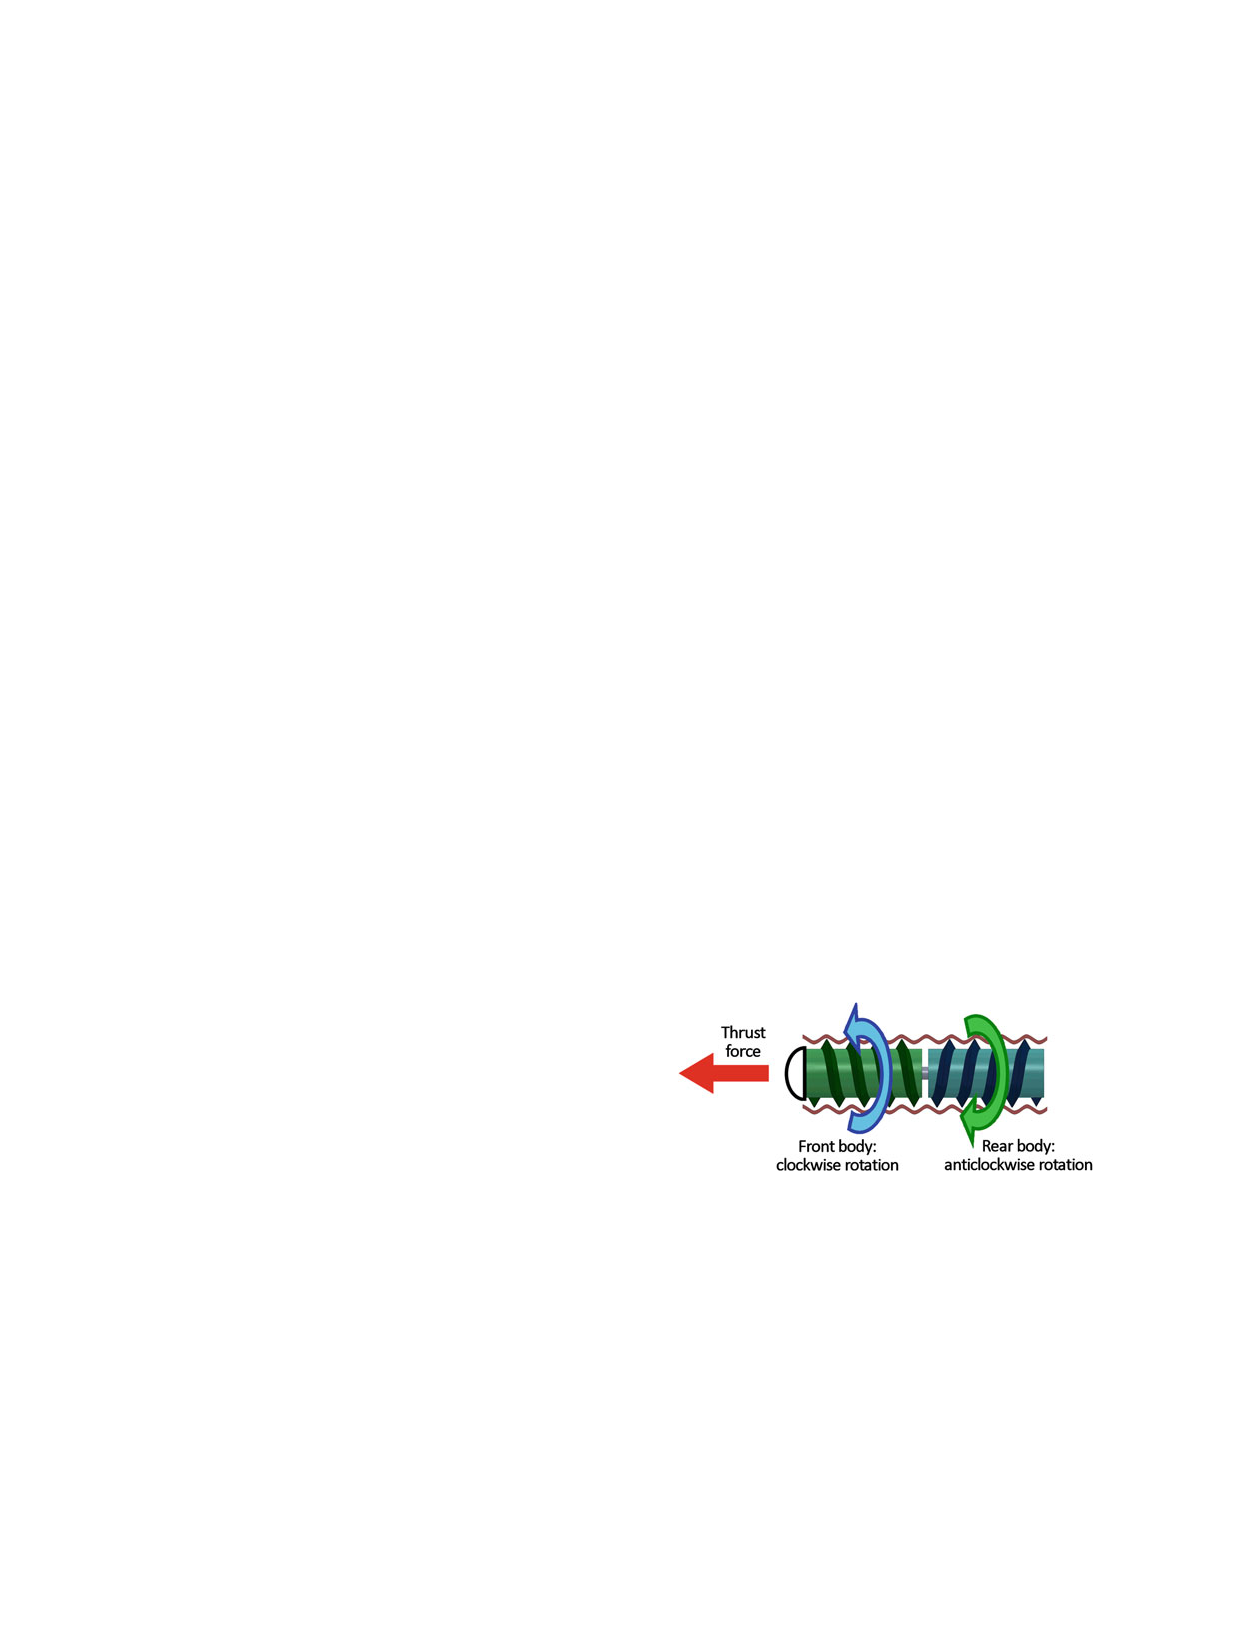
\includegraphics[width=2in]{Figures/ColonEndoscope-MotionPrinciple}
\hfill
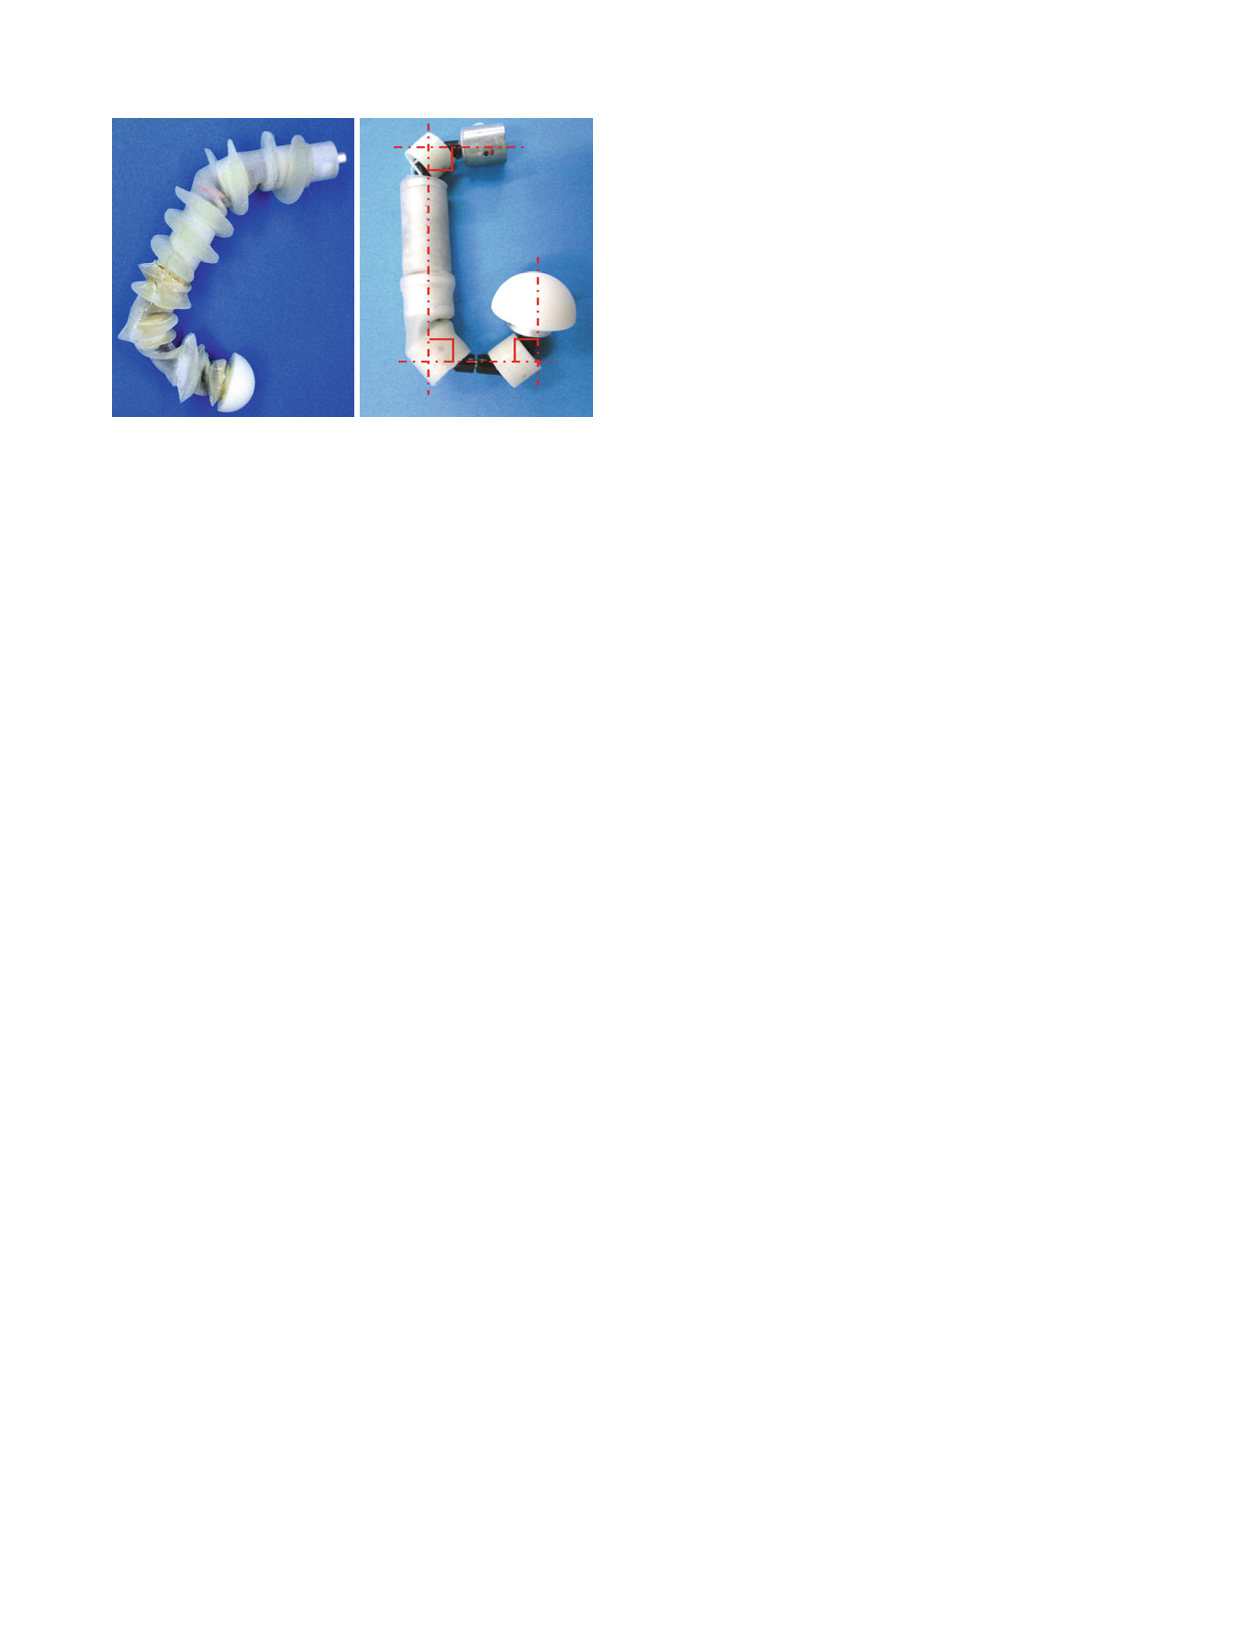
\includegraphics[width=1.5in]{Figures/ColonEndoscope-Model}
\hfill
\mbox{}

\ec

\bcol
\col
\pgfputat{\pgfxy(1.2,-0.5)}{\pgfbox[left,top]{
\includegraphics<+->[width=1.5in]{Figures/ColonEndoscope-SwineColon}
}}
\col
%\scaletext{0.7}{1}{
{\small
\bi
\item<+-> State-discretization: torque (9), movement (5)
\item<.-> Actions: voltage discretized to 5 levels
\item<.-> Reward: $1$ upon reaching waypoints (almost)
\item<.-> Using $\epsilon$-greedy with adaptive $\epsilon$
\ei
}
%}
\ecol

\note{
\bin
\item Input voltage is adjusted automatically by the robot, through the use of reinforcement learning, determining speed and direction (forward or backward).
\item
Results: Experiments were performed both in-vitro and in-vivo, showing the feasibility of the robot. The device is capable of moving in a slippery environment, and reinforcement learning algorithms such as Q-learning and SARSA can obtain better results than simply applying full tension to the robot.
 \item
Conclusions: This self-propelled robotic endoscope has potential as an alternative to current fibre optic colonoscopy examination methods, especially with the addition of new sensors under development.
 \ei
 }
}

\animframen{Results}
{
\bc
\includegraphics<+->[width=\textwidth]{Figures/ColonEndoscope-QLearning}
\ec
\note{
\bin
\item Input voltage is adjusted automatically by the robot, through the use of reinforcement learning, determining speed and direction (forward or backward).
\item
Results: Experiments were performed both in-vitro and in-vivo, showing the feasibility of the robot. The device is capable of moving in a slippery environment, and reinforcement learning algorithms such as Q-learning and SARSA can obtain better results than simply applying full tension to the robot.
 \item
Conclusions: This self-propelled robotic endoscope has potential as an alternative to current fibre optic colonoscopy examination methods, especially with the addition of new sensors under development.
 \ei
 }

}

\subsection{Fitted $Q$-iteration}

\begin{frame}[squeeze]
\frametitle{Fitted $Q$-iteration}
        \begin{algorithmic}[1]
        \Statex \mbox{} \hspace*{-2em} {\bf function} \Call{FittedQ}{$D,\theta$} 
	\Statex \mbox{} \hspace*{-2em} \textbf{Input:} $D = ( (\St_i,\Action_i,\Reward_{i+1},\Nextstate_{i+1});i =1,\ldots,n)$ is a list of transitions, $\theta$ are the regressor parameters
	\State $S \gets []$ \Comment{Create empty list}
	\For{$i=1 \to n$}
		\State $T \gets \Reward_{i+1} + 
					\max_{\nextaction\in\Actions} \mbox{\sc predict}(  (\Nextstate_{i+1},\nextaction), \theta)$ \Comment{Target at $(\St_i,\Action_i)$}
		\State $S \gets \Call{append}{ S,  \langle (\St_i,\Action_i), T \rangle}$ 
	\EndFor
	\State $\theta \gets \Call{regress}{S}$
	\State \Return $\theta$
	\end{algorithmic}
	\begin{block}{Caveat}
	The algorithm might diverge/become unstable
	To prevent this 
	\bi
	\item one might use a special regressor (``averager'') 
	\item one could use a powerful regressor such that  $\sup_{Q\in\FF} \| \Pi_{\FF} T^* Q - T^* Q\|$ is small
	\ei
	\end{block}
	\note{
		\bin
		\item Goal is to overcome the slow propagation of information
		\item Increased computational, storage cost
		\item Previous analysis applies (comparing first-order and least-squares type methods)
		\ei
	}
\end{frame}

\myframen{Application: Controlling the speed of a DC motor \\
 \small \citep{HaRie07:ADPRL}}
{
\bcol[c]
\col
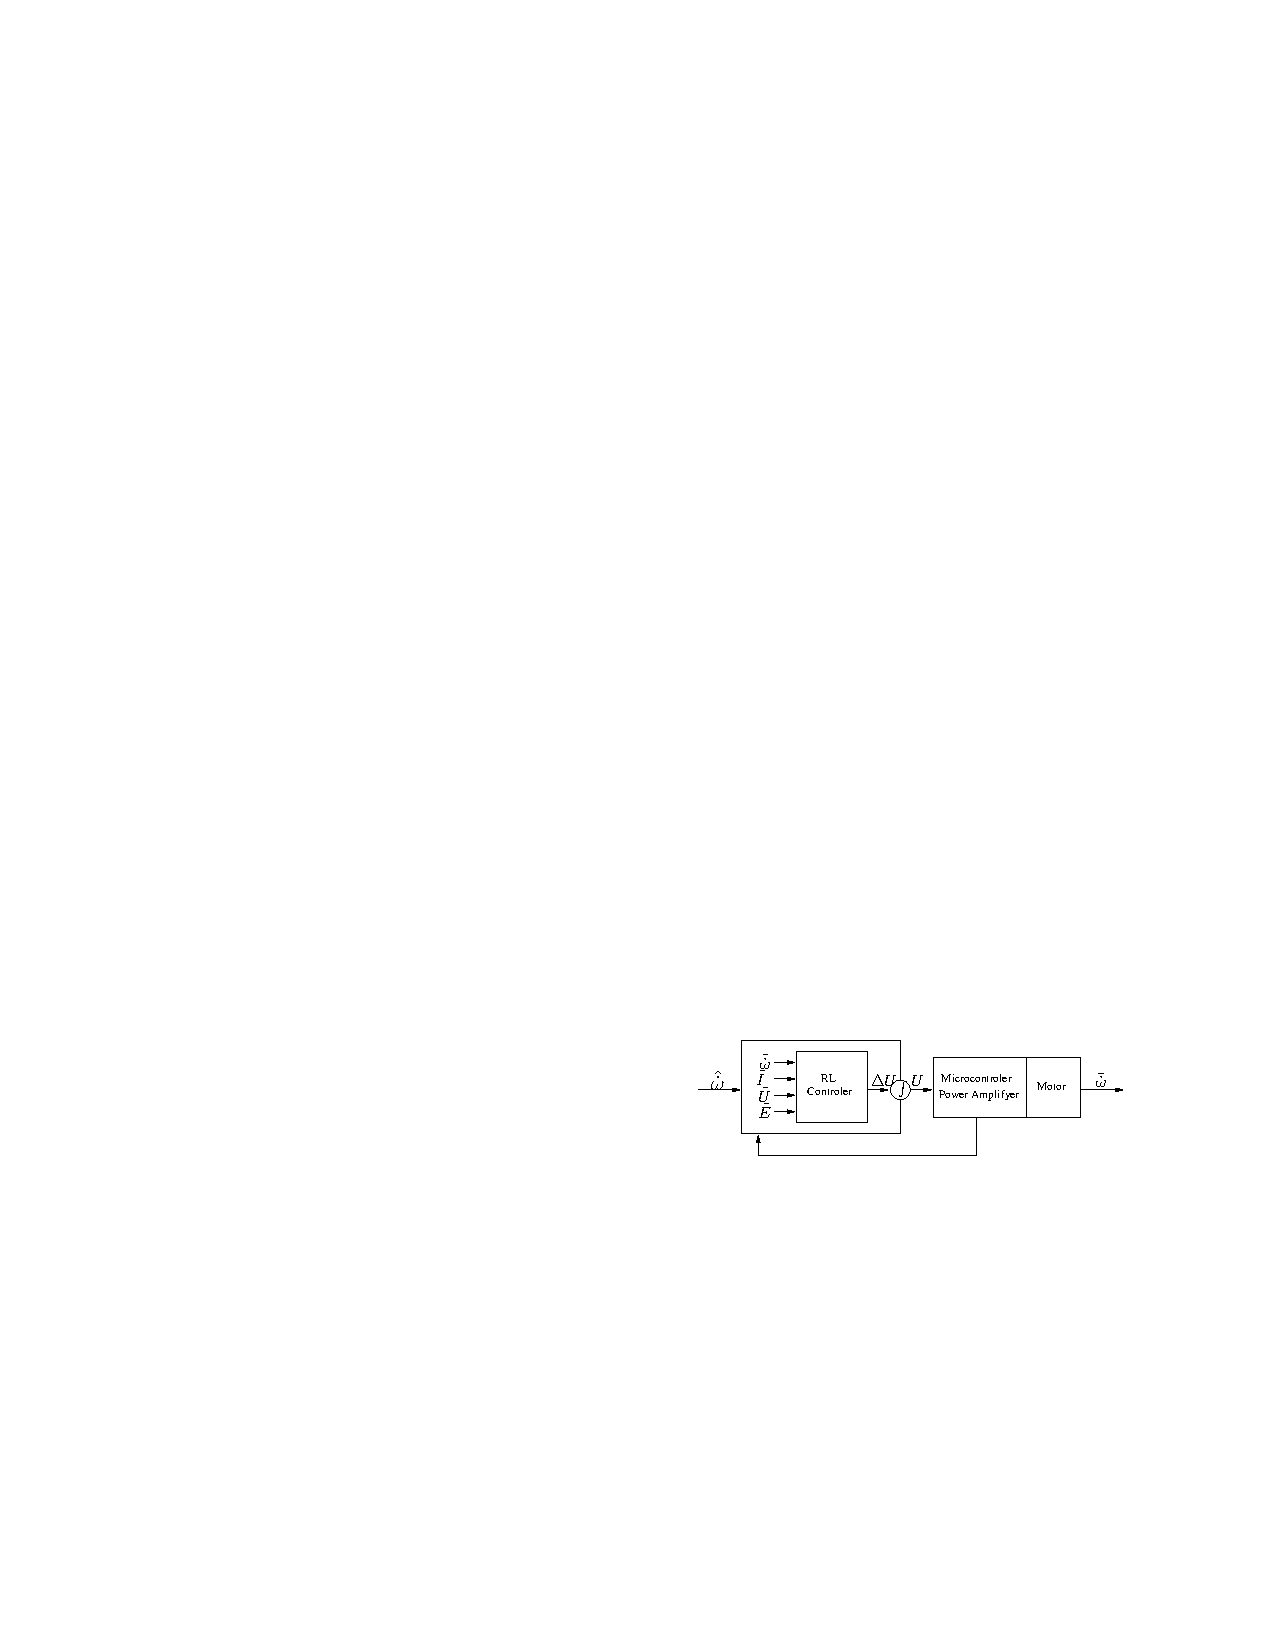
\includegraphics[width=\textwidth]{Figures/MAXON-DC-MOTOR-setup}
\col
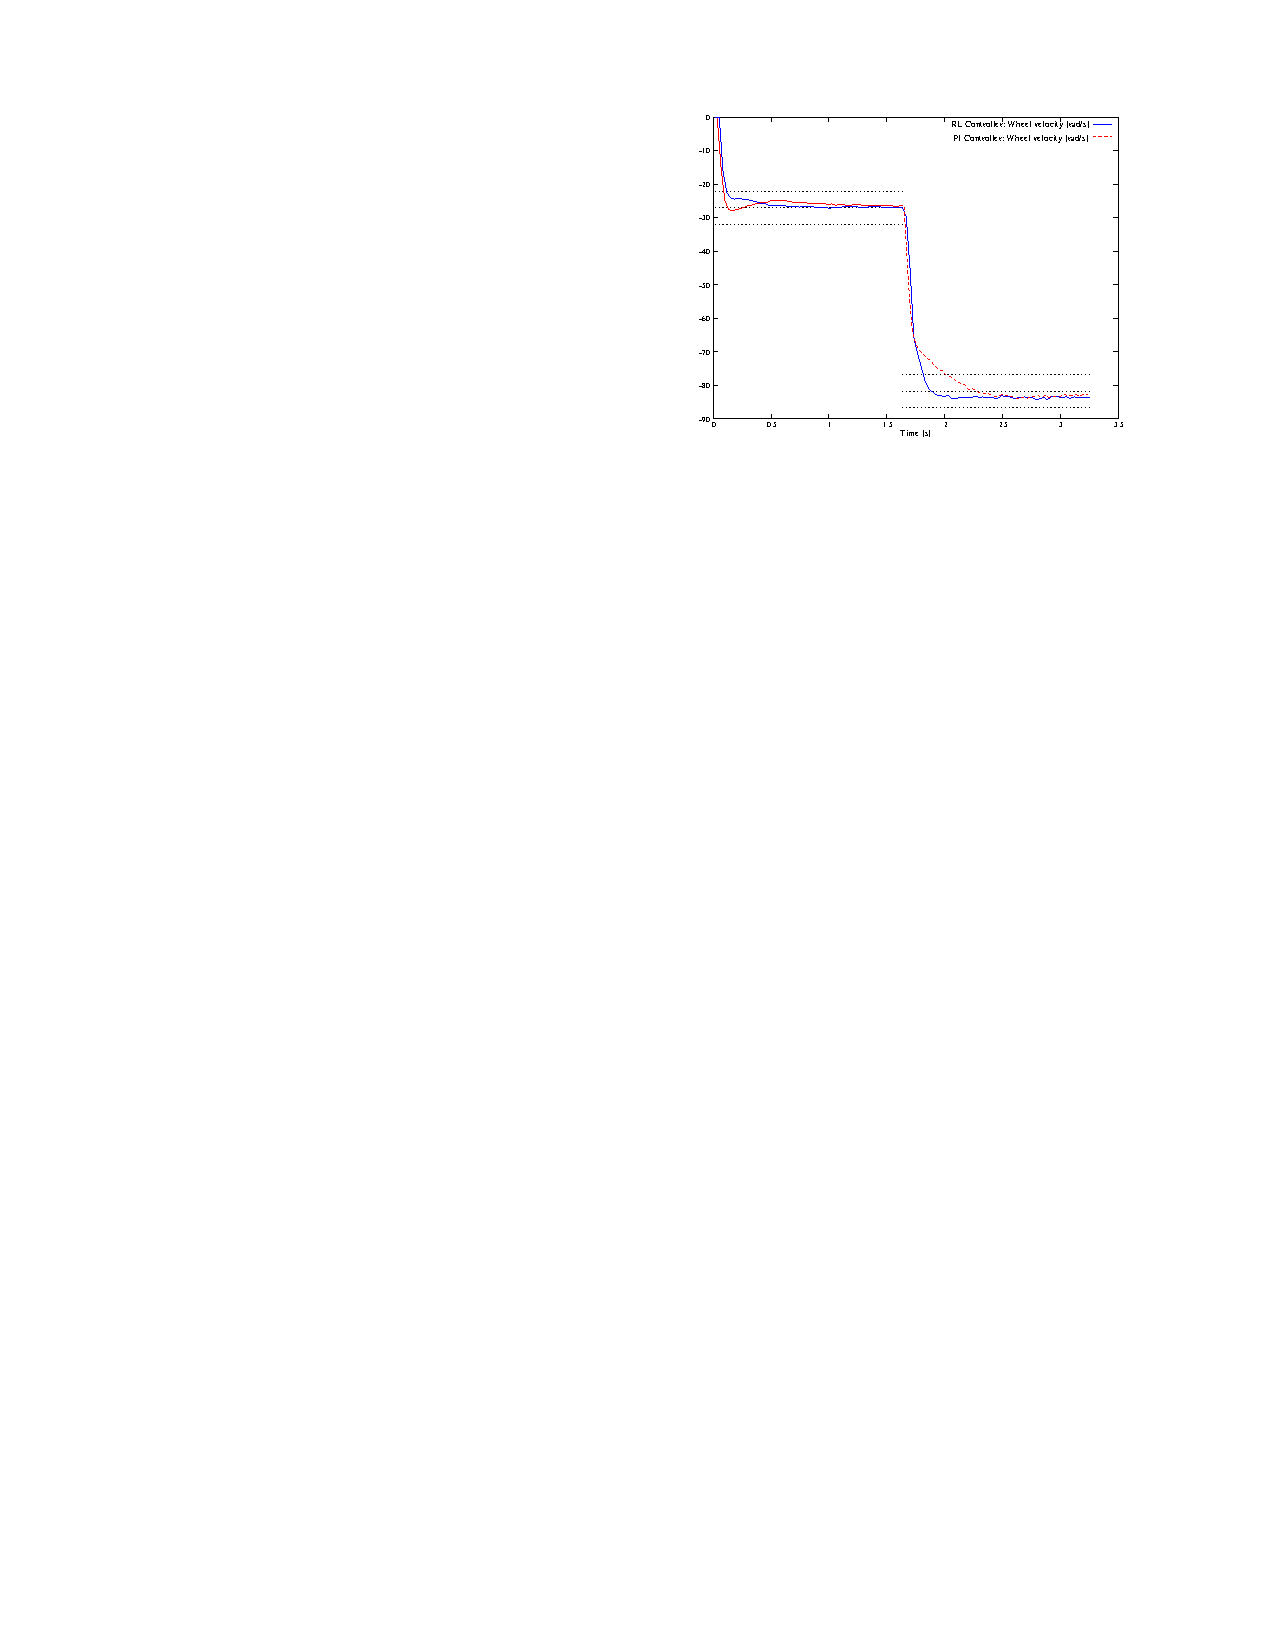
\includegraphics[width=0.7\textwidth]{Figures/MAXON-DC-MOTOR}
\ecol
\bi
\item Goal is to track a reference signal $\dot\omega_r = \dot\omega_r(t)$
\item Inputs:
{\tiny \bi
\item $I$ -- armature current
\item $\dot{\omega}$ -- current motor speed
\item $U$ -- actual voltage
\item $E = \dot\omega_r - \dot{\omega}$ -- tracking error
\ei}
\item Action: $\Delta U \in \{ -0.3, -0.1, -0.01, 0.0, 0.01, 0.1, 0.3 \}$
\item Reward: $-1$ if $E$ is big
\item Less than $5$ minutes of data is needed, $\Delta t = 33 \mathrm{ms}$
\ei
\note{
\bin
\item Goal is to learn a controller for regulating the speed of each single DC motor. 
\item The controller should be able to regulate the motor fast and accurately to arbitrary target speeds.
\item Learning will be based on interactions with the real motor only. 
\item Neither an analytical nor a simulated model will be used for learning.
\item One main reason for wanting a learning controller is the nonlinear behavior of the DC motor. 
\ei
}

}


\section{Actor-critic methods}

\animframen{The actor-critic architecture}
{
\begin{center}
\includegraphics<+->[width=0.5\textwidth]{Figures/ActorCritic}
\end{center}
}

\myframen{The actor-critic architecture}
{

\begin{block}{Implementation choices}
\bi
\item Critic: 
	\bi 
		\item Action-value functions or value functions? 
		\item What method?
	\ei
\item Actor:
	\bi
		\item With function approximation
		\bi
			\item What method?
		\ei
		\item Without function approximation
	\ei
	\item How to explore?
\ei
\end{block}

\putat{210}{-36}{\includegraphics<+->[width=1.9in]{Figures/ActorCritic}}
\note{
\bin
\item Even in simple cases convergence is hard to guarantee
\item ``Chattering'' is quite common
\item Sometimes performance degrades as times goes buy
\item The learning process is not so-well understood as in the case of prediction problems
\ei
}
}

\subsection{SARSA($\lambda$) with linear function approximation}
\begin{frame}[squeeze]
\frametitle{SARSA($\lambda$) with linear function approximation}

        \begin{algorithmic}[1]
        \Statex \mbox{} \hspace*{-2em} {\bf function} \Call{SARSALambdaLinFApp}{$\St,\Action,\Reward,\Nextstate,\Nextaction,\theta,z$} 
	\Statex \mbox{} \hspace*{-2em} \textbf{Input:} $\St$ is the last state, $\Action$ is the last action chosen,  $\Reward$ is the immediate reward received when transitioning to $\Nextstate$, where action $\Nextaction$ is chosen. $\theta\in \real^d$  is the parameter vector of the linear function approximation, $z\in \real^d$ is the vector of eligibility traces
	\State $\delta  \gets \Reward+\gamma \,\cdot\, \theta\ttop \phi[\Nextstate,\Nextaction] - \theta\ttop \phi[\St,\Action]$
	\State $z \gets \phi[\St,\Action] + \gamma \,\cdot\,\lambda\,\cdot\, z$
	\State $\theta \gets \theta + \alpha \,\cdot\,\delta\,\cdot\, z$
	\State \Return $(\theta,z)$
	\end{algorithmic}
%	\vspace*{1.82in}

\begin{alertblock}{}
\bc
SARSA $\equiv$\\
 current {\bf \underline S}tate,
 current {\bf \underline A}ction,
 next {\bf \underline R}eward,
 next {\bf \underline S}tate, and
 next {\bf \underline A}ction
%\vspace*{-0.1in}
\small \citep{rummery94b,rummery94}
\ec
\end{alertblock}
\note{
\bi
\item This is just TD($\lambda$) with action-value functions and linear function approximation.
\item Convergence (with a fixed policy!!!) follows from standard TD results
\item It is possible to use GTD2/TDC, too! (Maybe better, since there are expected to be less sensitive(?) to changing policies)
\item Another alternative is to use LSTDQ($\lambda$) and:
\bin
\item State features, $\psi:\States\ra\real^d$ s.t. $\sum_{\action\in\Actions} \pi(\action|\st) \phi(\st,\action)=0$, $\forall\st\in\States$
\item Define
 $Q_{\theta}(\st,\action) = \theta\ttop (\psi(\st)+\phi(\st,\action))$.
 \item
 Then $V_{\theta}(\st) = \sum_{\action\in\Actions}\pi(\action|\st) Q_\theta(\st,\action) = \theta\ttop \psi(\st)$.
 \item Setting $V_{t+1} = V_{\theta}(\Nextstate_{t+1})$ 
 does not introduce any bias, 
 while it is expected to reduce variance
\item ``Compatible function approximation''
% \citep{PetVijSch03,PeSch08}.%
\ei
\ei
}
\end{frame}


\if0
Modern DRAM systems consist of dual in-line memory mod- ules (DIMMs), which are composed of multiple DRAM chips put together to obtain a wide data interface. Each DRAM chip is organized as multiple independent memory banks. Each bank is a two-dimensional array organized as rows ? columns.
Only a single row can be accessed in each bank at any given time. Each bank contains a row buffer that stores the row that can be accessed. To access a location in a DRAM bank, the memory controller must first make sure that the row is in the row buffer. An activate command brings the row whose address is indicated by the address bus from the memory array into the row buffer. Once the row is in the row buffer, the controller can issue read or write commands to access a column whose address is indicated by the address bus. Each read or write command transfers multiple columns of data, specified by a programmable burst length parameter. To access a different row, the controller must first issue a precharge command so that the data in the row buffer is written back to the memory array. After the precharge, the controller can issue an activate command to open the new row it needs to access.
The memory controller accepts cache misses and write-back requests from the processor(s) and buffers them in a memory transaction queue. The controller�s function is to satisfy such re- quests by issuing appropriate DRAM commands while preserving the integrity of the DRAM chips. To do so, it tracks the state of each DRAM bank (including the row buffer), each DRAM bus, and each memory request. The memory controller�s task is complicated due to two major reasons.


First, the controller needs to obey all DRAM timing constraints to provide correct functionality. DRAM chips have a large number of timing constraints that specify when a command can be legally issued. There are two kinds of timing constraints: local (per-bank) and global (across banks due to shared resources between banks). An example local constraint is the activate to read/write delay, tRCD, which specifies the min- imum amount of time the controller needs to wait to issue a read/write command to a bank after issuing an activate com- mand to that bank. An example global constraint is the write to read delay, tWTR, which specifies the minimum amount of time that needs to pass to issue a read command to any bank after issuing a write command to any bank. State-of-the-art DDR2 SDRAM chips often have a large number of timing constraints that must be obeyed when scheduling commands (e.g., over 50 timing constraints in [26]).
Second, the controller must intelligently prioritize DRAM commands from different memory requests to optimize system performance. Different orderings and inter- leavings of DRAM commands result in different levels of DRAM throughput and latency [37]. Finding a good schedule is not an easy task as scheduling decisions have long-term consequences: not only can issuing a DRAM command prevent servicing other requests in subsequent DRAM cycles (due to timing constraints), but also the interleaving of requests from different cores (and therefore the future contents of the memory reference stream) is heavily influenced by which core�s blocking requests get serviced next (possibly unblocking the instruction window or the fetch unit of the requesting core, allowing it to generate new memory requests). Moreover, the ultimate benefit provided by a schedul- ing decision is heavily influenced by the future behavior of the processors, which certainly is not under the scheduler�s control.


Current memory controllers use relatively simple policies to schedule DRAM accesses. Rixner et al. [37] show that none of the fixed policies studied provide the best performance for all workloads and under all circumstances. However, the FR-FCFS (first-ready first-come first-serve) policy [36, 37] provides the best average performance. Among all ready commands, FR-FCFS prioritizes (1) column (CAS) commands (i.e., read or write com- mands) over row (RAS) commands (i.e., activate and precharge) in order to maximize the number of accesses to open rows, and (2) older commands over younger commands. Hence, FR-FCFS gives the highest priority to the oldest ready column command in the transaction queue. The goal of the FR-FCFS policy is to maximize DRAM throughput and minimize average request la- tency. However, FR-FCFS does not consider the long-term per- formance impact of either (1) prioritizing a column command over a row command, or (2) prioritizing an older command over a younger command.

\fi

\myframen{Application: DRAM command scheduling}
{
\begin{block}{Problem \citep{IpeMutMar08}}
\bcol[c]
\col
\bi
\item Goal: Optimize DRAM command scheduling policy to optimize performance
\item Tool: SARSA(0) with CMAC (tile coding)
\item Observations: Transaction queue
\item Actions: Candidate scheduling commands
\item Reward: $1$ for read/write, $0$ for others (e.g. precharge, activate,..)
\ei
\col
\includegraphics<+->[width=\textwidth]{Figures/DRAM-Application}
\ecol
\end{block}
}

\myframen{Application: DRAM command scheduling}
{
\bcol[c]
\col[0.6\textwidth]
\bc
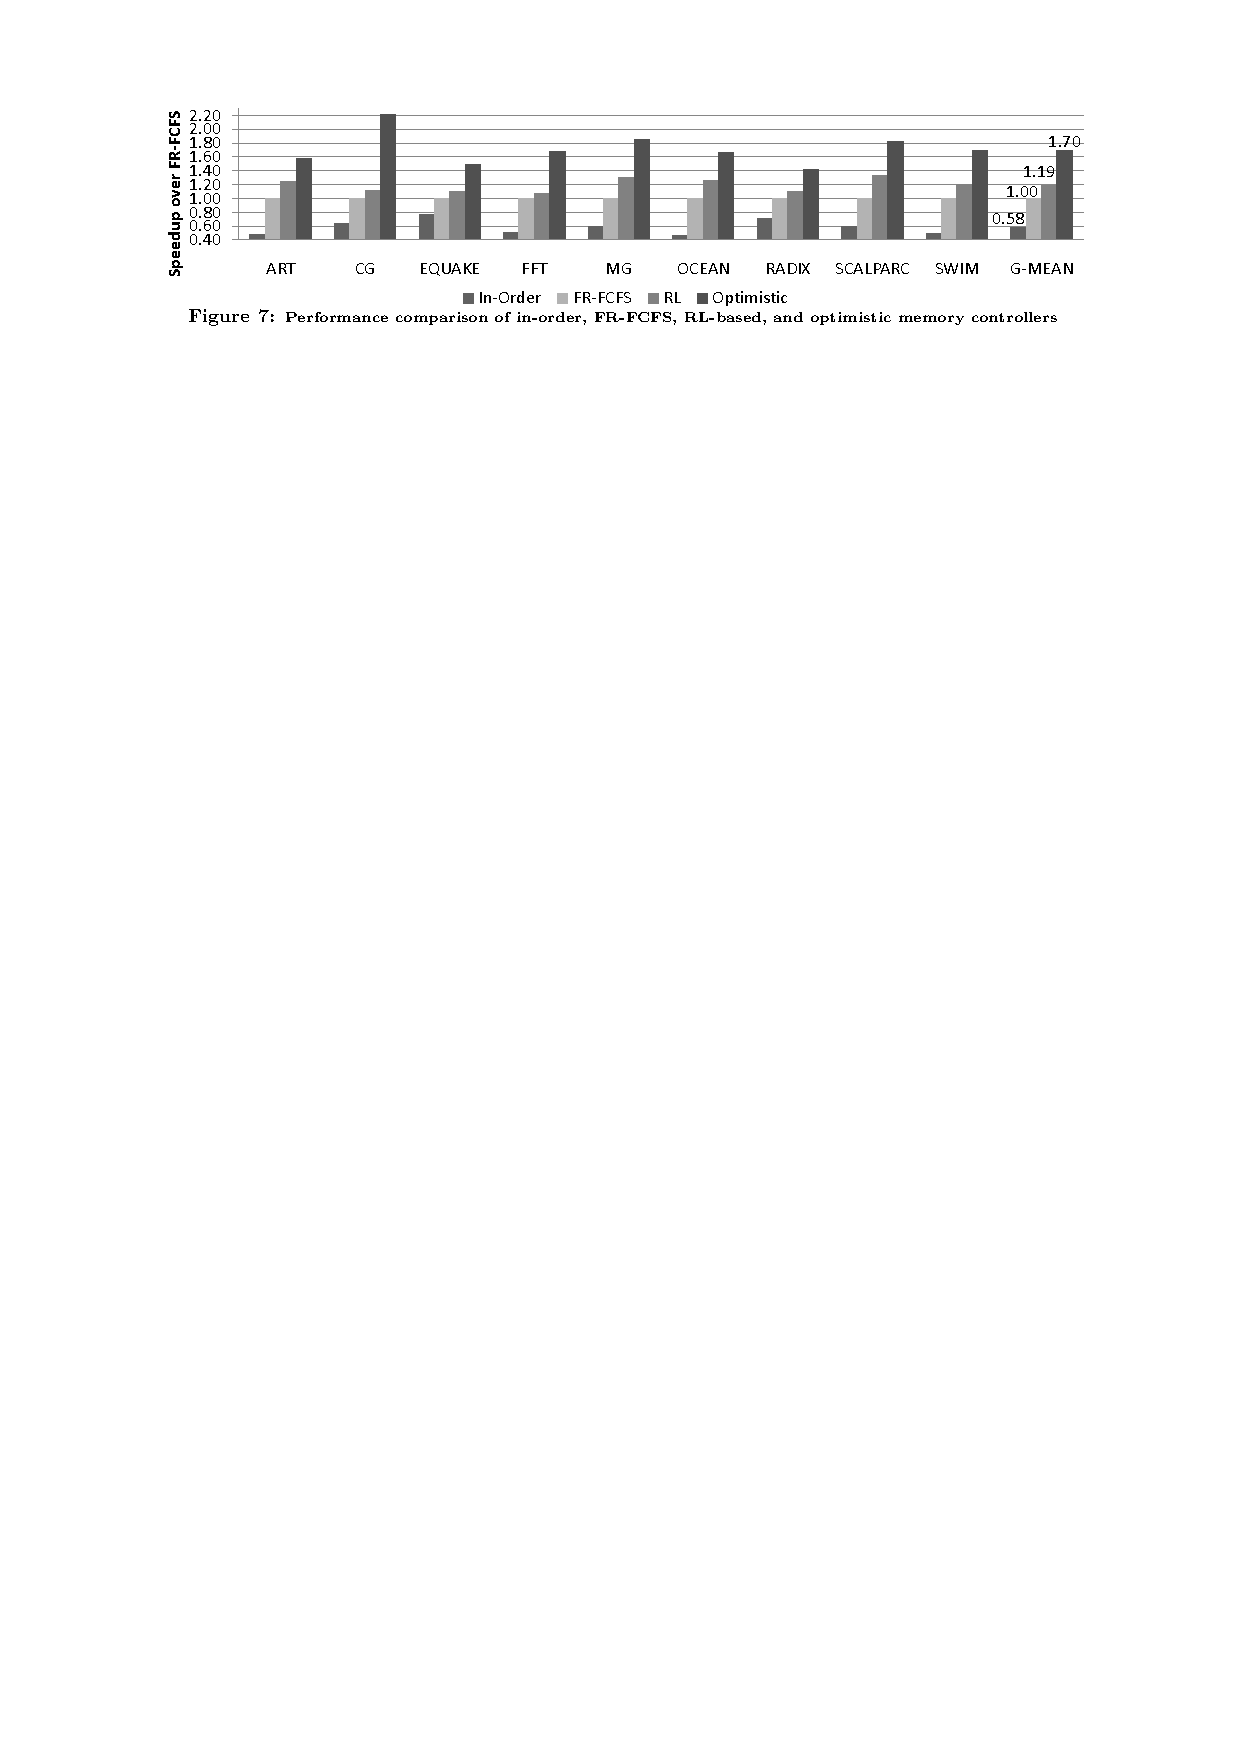
\includegraphics[width=\textwidth]{Figures/DRAM-speedup}

\bigskip
\bigskip
\bigskip
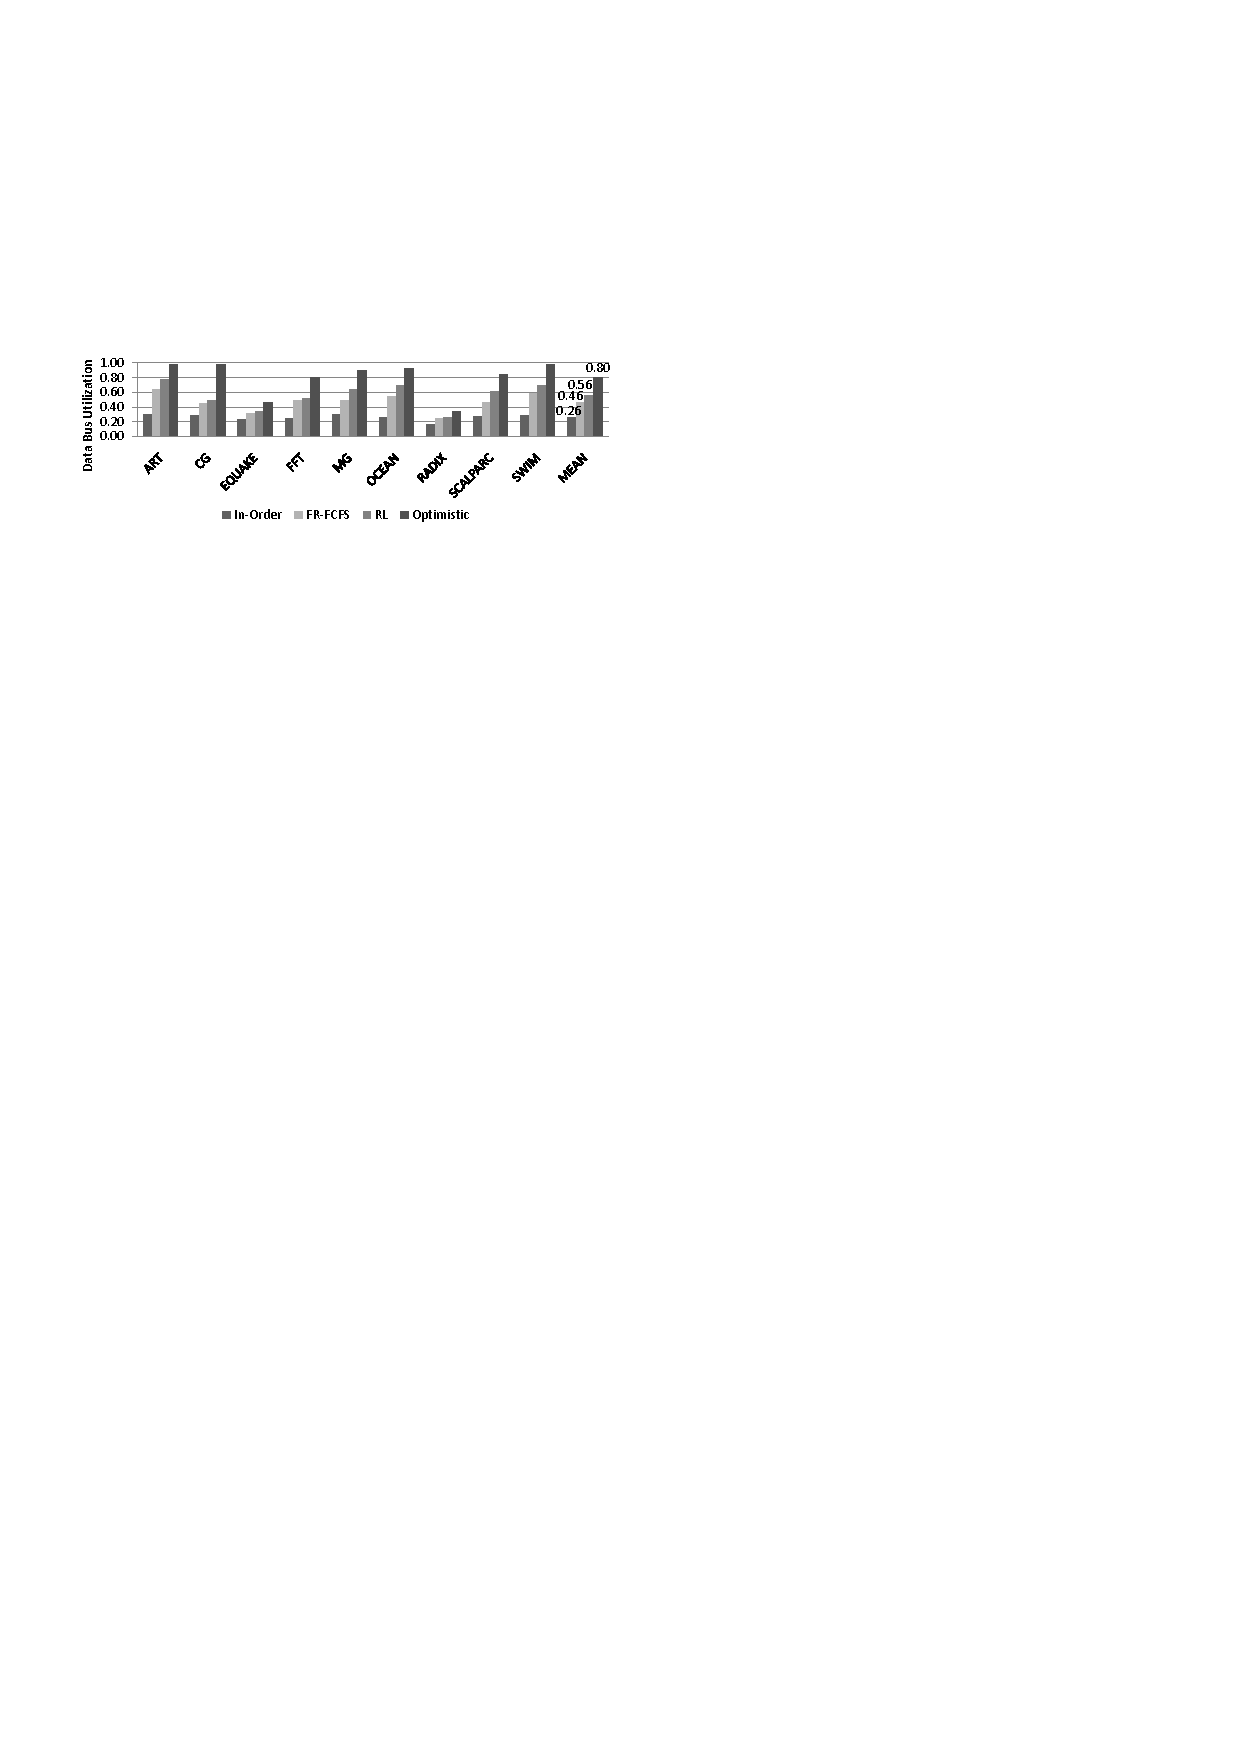
\includegraphics[width=\textwidth]{Figures/DRAM-utilization}

\ec
\col[0.4\textwidth]
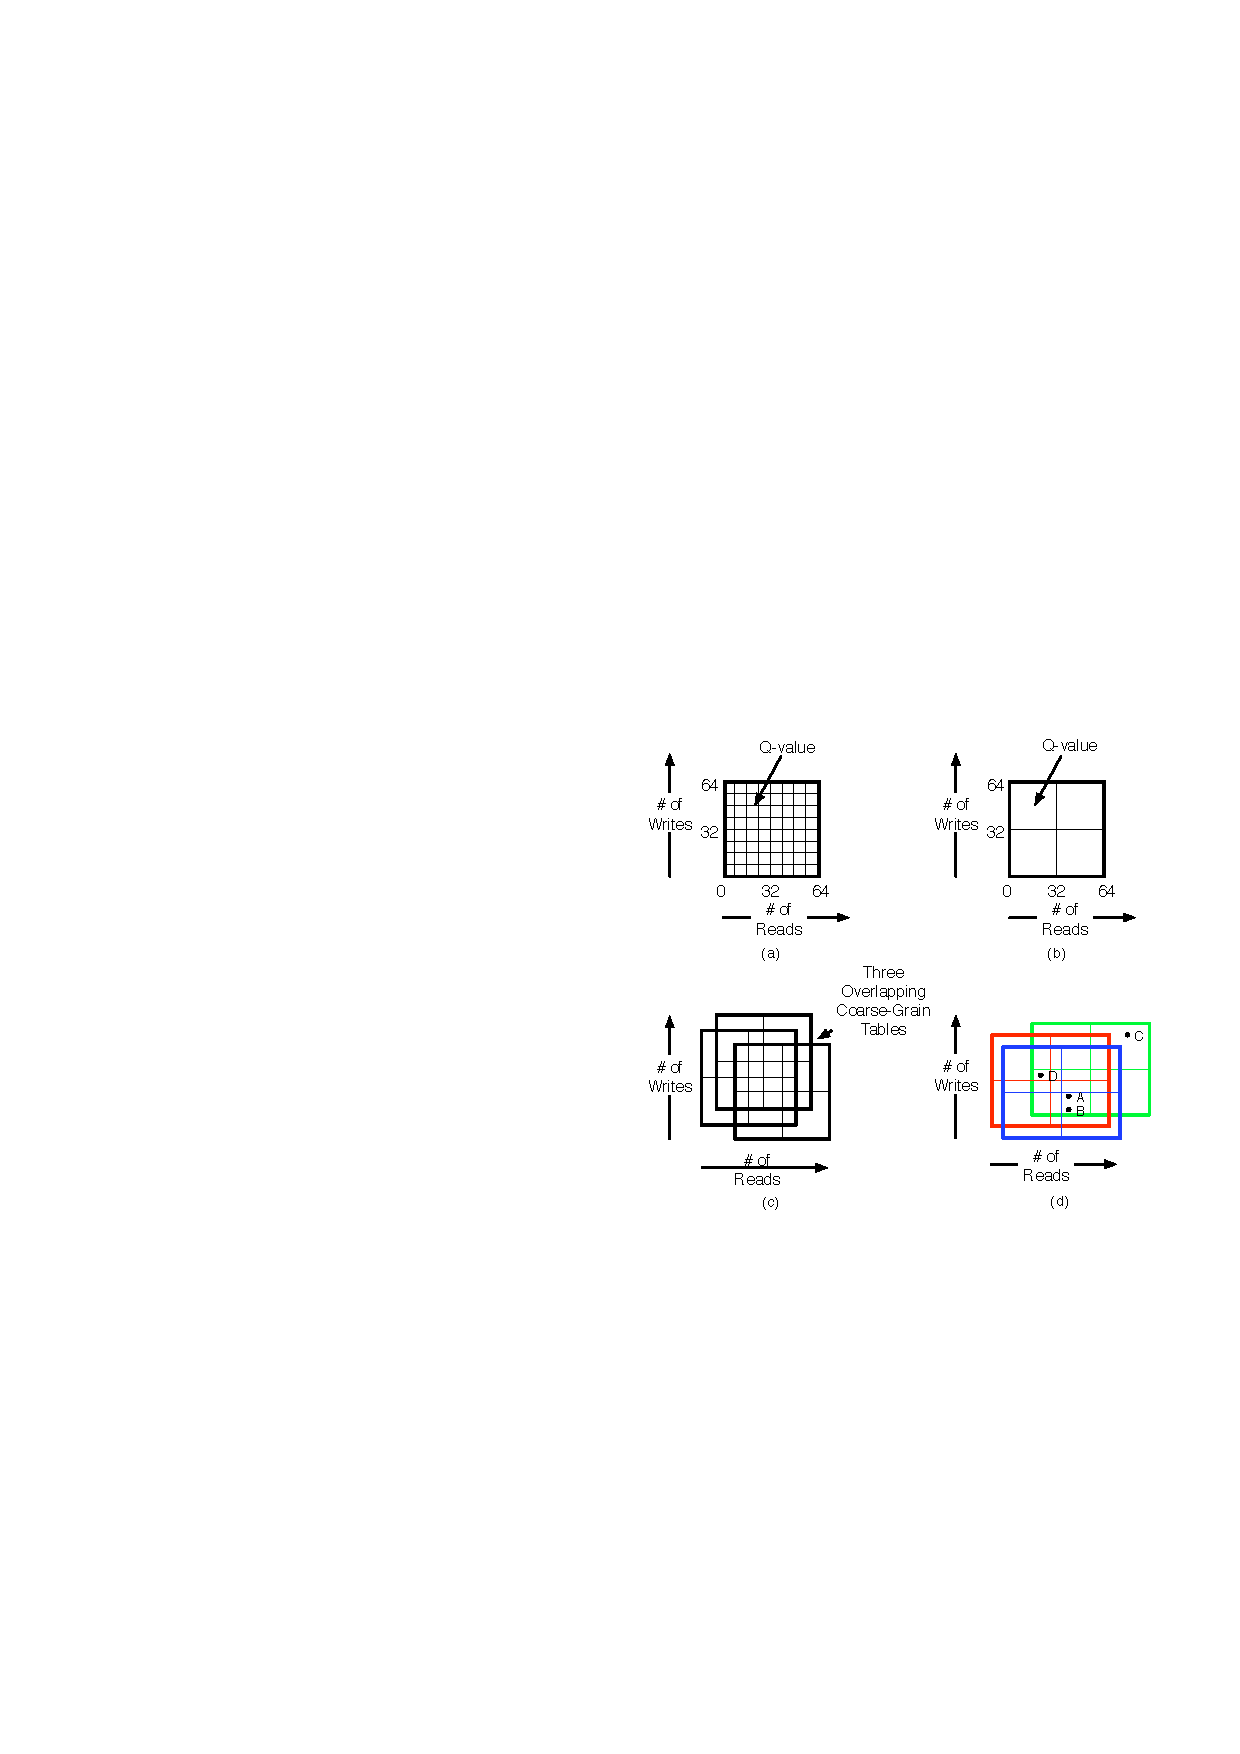
\includegraphics[width=\textwidth]{Figures/DRAM-CMAC}
\ecol

\note{
They have a hardware implementation!!

First graph: How much speedup compared to the industry standard. ``Optimistic'' is unrealizable (provided an upper bound)

Second graph: Explains how the speedup is achieved (better utilization of data bandwidth)
\begin{quotation}
\tiny
We have presented a new approach to designing memory controllers that operate using the principles of reinforcement learning (RL). An RL-based, self-optimizing memory controller continuously and automatically adapts its DRAM command scheduling policy based on its interaction with the system to optimize performance. As a result, it can utilize DRAM bandwidth more efficiently than a traditional controller that employs a fixed scheduling policy. Our approach also reduces the human design effort for the memory controller because the hardware designer does not need to devise a scheduling policy that works well under all circumstances.

On a 4-core CMP with a single-channel DDR2-800 memory subsystem (6.4GB/s peak bandwidth in our setup), the RL- based memory controller improves the performance of a set of parallel applications by 19\% on average (up to 33\%) and DRAM bandwidth utilization by 22\% on average, over a state-of-the-art FR-FCFS scheduler. 
This improvement effectively cuts in half the performance gap between the single-channel configuration and a more expensive dual-channel DDR2-800 subsystem with twice peak bandwidth. When applied to the dual-channel sub- system, the RL-based scheduler delivers an additional 14\% performance on average (up to 34\%). 
We conclude that RL-based self-optimizing memory controllers provide a promising way to efficiently utilize the DRAM memory bandwidth available in a CMP.
\end{quotation}
}
}

\subsection{Policy gradient}
\animframen{Policy gradient}
{
\bi
\item Fix $\Pi = (\pi_{\aparam};\aparam\in\real^{\dimaparam})$ % -- class of stochastic stationary policies, smooth parameterization
%Here $g_\aparam$ and $\Sigma_\aparam$ are parametric functions (e.g., these could be neural networks).
\item \alert{Goal}:
	\[
	\argmax_{\aparam} \perf_\aparam = ?
	\]
\item Choices for  $\perf_\aparam$:
	\bi
		\item 
		 $\perf_\aparam = \EE{V^{\pi_{\aparam}}(\St_0) }$,
		 $\St_0 \sim \mu$
		\item When $\mu$ is the stationary distribution of $\pi$ ($\mu = \mu_\pi$),
			 the two performance measures become the same, apart from a constant factor
	\ei
\ei
\note{
\bin
	\item Finite action space;
	 \alert{Gibbs policies}:
	\[
	\pi_\aparam(\action|\st) = \frac{ \exp( \aparam\ttop \xi(\st,\action) )}{\sum_{\action'\in \Actions}  \exp( \aparam\ttop \xi(\st,\action') ) },
	\qquad \st\in\States,\action\in\Actions.
	\]
%	Here $\xi:\SA\ra \real^{\dimaparam}$ is an appropriate feature-extraction function.
	\item Infinite action space; $\Actions\subset \real^{\dimaction}$, \alert{Gaussian policies}:
	\[
	\pi_\aparam(\action|\st) = 
	\frac{\exp\Bigl(
	- (\action - g_\aparam(\st,\action))\ttop \Sigma_\aparam^{-1}(\st,\action) \,(\action-g_\aparam(\st,\action)
	\Bigr)}
	{ \sqrt{ ( 2\pi)^{\dimaction} {\rm det}(\Sigma_\aparam(\st,\action))} }.
	\]
\item[]
Care must be taken to ensure that $\Sigma_\aparam$ is positive definite. For simplicity, $\Sigma_\aparam$ is often taken to be $\Sigma_\aparam=\beta I$ with some $\beta>0$.
\ei
}
}

\animframen{Policy gradient theorem}
{
\begin{block}{Assumption}
The Markov chain resulting from following any policy $\pi_\aparam$ is ergodic, regardless of the choice of $\aparam$.
\end{block}
\bi
\item How to estimate  the gradient of $\perf_\aparam$?
\item
Let $\psi_\aparam:\SA \ra \real^{\dimaparam}$ be the \alert{score function}  underlying $\pi_\aparam$:
\[
\scorefun_\aparam(\st,\action) = \pscorefunp{\action|\st},\qquad (\st,\action)\in \SA.
\]
\item
Define
\[
G(\aparam) =
  \bigl( Q^{\pi_\aparam}(\St,\Action) - h(\St) \bigr)\, \, \scorefun_\aparam(\St,\Action),
\]
where $(\St,\Action)\sim \mu_{\pi_\aparam}$ .
% a sample from the stationary state-action distribution underlying policy $\pi_\aparam$;
\item Let
 $Q^{\pi_\aparam}$ be the action-value function of $\pi_\aparam$ and
 $h$ is an arbitrary bounded function.
 \ei
}
\animframen{Policy gradient theorem II}
{
 \begin{Theorem}[Policy gradient theorem]
%(see, e.g., \citealp{BhaSuGhaLee09} %\citet{MarTsi03}  and the references therein),
\bc
$\nabla_\aparam \perf_\aparam = \EE{ G(\aparam)}.$
\ec
 \end{Theorem}
\begin{Corollary}
Let  $(\St_t,\Action_t)\sim \mu_{\pi_{\aparam_t}}$, and assume
\beq
\label{eq:qpg}
\EE{ \hQ_t(\St_t,\Action_t) \scorefun_{\aparam_t}(\St_t,\Action_t) }
=
 \EE{ Q^{\pi_{\aparam_t}}(\St,\Action)  \scorefun_{\aparam_t}(\St_t,\Action_t) }.
 \tag{Q-PG}
\eeq
Then
\beq
\begin{split}
\aparam_{t+1} = \aparam_t + \beta_t \,
  \bigl( \hQ_t(\St_t,\Action_t)- h(\St_t) \bigr)\, \, \scorefun_\aparam(\St_t,\Action_t)
\end{split}
\label{eq:pga}
\eeq
 implements stochastic gradient ascent.
\end{Corollary}
\note{
\bi
\item In the case of Gibbs policies, the score function takes the form $\scorefun_\aparam(\st,\action) = \xi(\st,\action) - \sum_{\action'\in \Actions} \pi_\aparam(\action'|\st) \xi(\st,\action')$.
\item $\mu_{\pi_\aparam}$ is the stationary policy underlying $\pi_\aparam$
\ei
}
}

\animframesqn{Compatible function approximation}
{
\begin{block}{Compatible function approximation}
	Choose the feature-extraction function to be the score function underlying the policy class:
	\[
		Q_\theta(\st,\action) = \theta\ttop \scorefun_\aparam(\st,\action), \qquad (\st,\action)\in \SA.
	\]
	%This choice of the function approximation method is called {\em compatible} with the policy parameterization.
\end{block}

\begin{block}{Note}
	The basis functions change when $\aparam$ changes!
\end{block}

\begin{Theorem}
	Let 
		$\theta_*(\aparam) = \argmin_{\theta} \EE{ (Q_\theta(\St,\Action)-Q^{\pi_\aparam}(\St,\Action))^2}$.
	Then $Q_{\theta_*(\aparam)}$ satisfies \eqref{eq:qpg} and
	\[
		\aparam_{t+1} = \aparam_t + \beta_t \,
		  \bigl( \hQ_{\theta_*(\aparam_t)}(\St_t,\Action_t)- h(\St_t) \bigr)\, \, \scorefun_\aparam(\St_t,\Action_t)
	\]
	implements stochastic gradient ascent.
\end{Theorem}

\note{
\vspace*{-0.1in}
Proof of the theorem:
Substituting  $Q_\theta$ for $\hQ_t$ in \eqref{eq:qpg}, we get
\[
\EE{  \scorefun_{\aparam_t}(\St_t,\Action_t) \scorefun_{\aparam_t}(\St_t,\Action_t)\ttop }
\theta
=
 \EE{ Q^{\pi_{\aparam_t}}(\St_t,\Action_t)  \scorefun_{\aparam_t}(\St_t,\Action_t) }.
\]
Define $F_ \aparam = \EE{  \scorefun_{\aparam}(\St,\Action) \scorefun_{\aparam}(\St,\Action)\ttop }$,
$g_ \aparam = \EE{ Q^{\pi_{\aparam}}(\St,\Action)  \scorefun_{\aparam}(\St,\Action) }$
and
let
$\theta_*(\aparam)$ be the solution to the linear system of equations
\[
F_ \aparam \,\theta = g_\aparam.
\]
When this equation holds, $Q_{\theta_*(\aparam_t)}$ satisfies~\eqref{eq:qpg}.
Notice that $\theta_*(\aparam)$ is the parameter that minimizes the mean-squared error
 \[
 \EE{ (Q_\theta(\St,\Action)-Q^{\pi_\aparam}(\St,\Action))^2}.
 \]
\alert{Algorithm}: Use SARSA($1$) on a faster timescale (slave) and the update rule of the theorem
on a slower timescale. This gives a provably convergent policy-gradient method.
}
}

\subsection{Actor-critic with SARSA(1)}
\begin{frame}
\frametitle{Actor-critic with SARSA(1)}

        \begin{algorithmic}[1]
        \Statex \mbox{} \hspace*{-2em} {\bf function} \Call{SARSAActorCritic}{$\St$} 
		\Statex \mbox{} \hspace*{-2em} \textbf{Input:} $\St$ is the current state
		\State $\aparam,\theta,z \gets 0$
		\State $\Action \gets \action_1$ \Comment{Pick any action}
		\Repeat
		\State $(\Reward,\Nextstate) \gets \Call{ExecuteInWorld}{\,\Action\,}$
		\State $\Nextaction \gets \Call{Draw}{ \pi_\aparam(\Nextstate,\cdot) }$
		\State $(\theta,z) \gets \Call{SARSALambdaLinFApp}{\St,\Action,\Reward,\Nextstate,\Nextaction,\theta,z}$
		\State
		\Comment{Use $\lambda=1$ and $\alpha\gg \beta$}
		\State $\psi \gets \frac{\partial}{\partial\aparam} \log \pi_{\aparam}(\St,\Action)$
		\State $v \gets \Call{sum}{\,\pi_\aparam(\Nextstate,\cdot\,) \cdot \theta\ttop \phi[\St,\cdot\,]\,}$
		\State $\aparam \gets \aparam +
		 \beta \cdot \left( \theta\ttop \phi[\St,\Action] - v \right) \cdot \psi$
		 \label{line:cfaccapu}
		\State $\St \gets \Nextstate$
		\State $\Action \gets \Nextaction$
		\Until{\texttt{True}}
		\end{algorithmic}

\note{ 
	This just shows the implementation of the algorithm motivated by the Theorem on the last slide.
	
	\citet{KonTsi03} proved that (under some regularity conditions) 
	$\liminf_{t\ra\infty} \nabla_\aparam \rho_{\aparam_t}=0$ holds almost surely if the average-cost version of SARSA(1) is used to update $\theta_t$. 
	They have also shown that if SARSA($\lambda$) is used 
	and $m_\lambda = \liminf_{t\ra\infty} \nabla_\aparam \rho_{\aparam_t}$
	then $\lim_{\lambda\ra 1 }m_\lambda=0$.

}
\end{frame}

\subsection{Natural actor-critic}

\begin{frame}[squeeze]
\frametitle{Natural actor-critic}

        \begin{algorithmic}[1]
        \Statex \mbox{} \hspace*{-2em} {\bf function} \Call{\only<1|handout:0>{SARSAActorCritic}\only<2->{\alert{NAC}}}{$\St$} 
	\Statex \mbox{} \hspace*{-2em} \textbf{Input:} $\St$ is the current state
	\State $\aparam,\theta,z \gets 0$, $\Action \gets \action_1$ \Comment{Pick any action}
	\Repeat
		\State $(\Reward,\Nextstate) \gets \Call{ExecuteInWorld}{\,\Action\,}$
		\State $\Nextaction \gets \Call{Draw}{ \pi_\aparam(\Nextstate,\cdot) }$
		\State $(\theta,z) \gets \Call{SARSALambdaLinFApp}{\St,\Action,\Reward,\Nextstate,\Nextaction,\theta,z}$
		\State
		\Comment{Use $\lambda=1$ and $\alpha\gg \beta$}
		\State $\psi \gets \frac{\partial}{\partial\aparam} \log \pi_{\aparam}(\St,\Action)$
		\State $v \gets \Call{sum}{\,\pi_\aparam(\Nextstate,\cdot\,) \cdot \theta\ttop \phi[\St,\cdot\,]\,}$
		\State $\aparam \gets \aparam + 
		 	\only<1|handout:0>{\beta \cdot \left( \theta\ttop \phi[\St,\Action] - v \right) \cdot \psi}
			\only<2->{\alert{\beta \cdot \theta} }
			$
		 \label{line:cfaccapu}
		\State $\St \gets \Nextstate$
		\State $\Action \gets \Nextaction$
	\Until{\texttt{True}}
	\end{algorithmic}

\note{Note the one line difference. Is not it nice that the update gets simplified? But does it work?}
\end{frame}

\animframe{Natural actor-critic}
{
\bi
	\item We have $\theta_*(\aparam) = F_\aparam^{-1} \nabla_\aparam \rho_\aparam$ for a suitable $F_\aparam$.
	\item[] $\Longrightarrow$ this is a stochastic \alert{pseudo}-gradient algorithm
	\item Better: This algorithm follows a (more) \alert{natural} gradient
	\bi
	\item Gradient in the space of policies: Avoiding plateaus 
	\item Covariant trajectories (insensensitive to reparameterizing $\pi_\aparam$)
	\ei
\ei

\note{
	\bin
	\item Pseudo-gradient, since
		 $\theta_*(\aparam)\ttop \nabla_\aparam \perf_\aparam  
			 = \nabla_\aparam \perf_\aparam\ttop F_\aparam^{-1}\nabla_\aparam \perf_\aparam > 0$
		unless $\nabla_\aparam \perf_\aparam=0$.
	\item Natural gradient: Not hard to prove, but we do not do it here
	\item There is no such thing as ``the'' natural gradient:
		\bin
		\item The choice of the gradient depends on the norm (distance) used:
		\item[] $f(x+h) - f(x) = f'(x) h + o( \|h\| )$, note the use of the norm!
		\item Should we use it? Opinion: It is a choice that is good to have.
		\item Also, it explains why some previously proposed algorithms work!
		\ei
	\ei
}
}

\myframen{Learning motor primitives with NAC -- Toy problems}
{
\bc
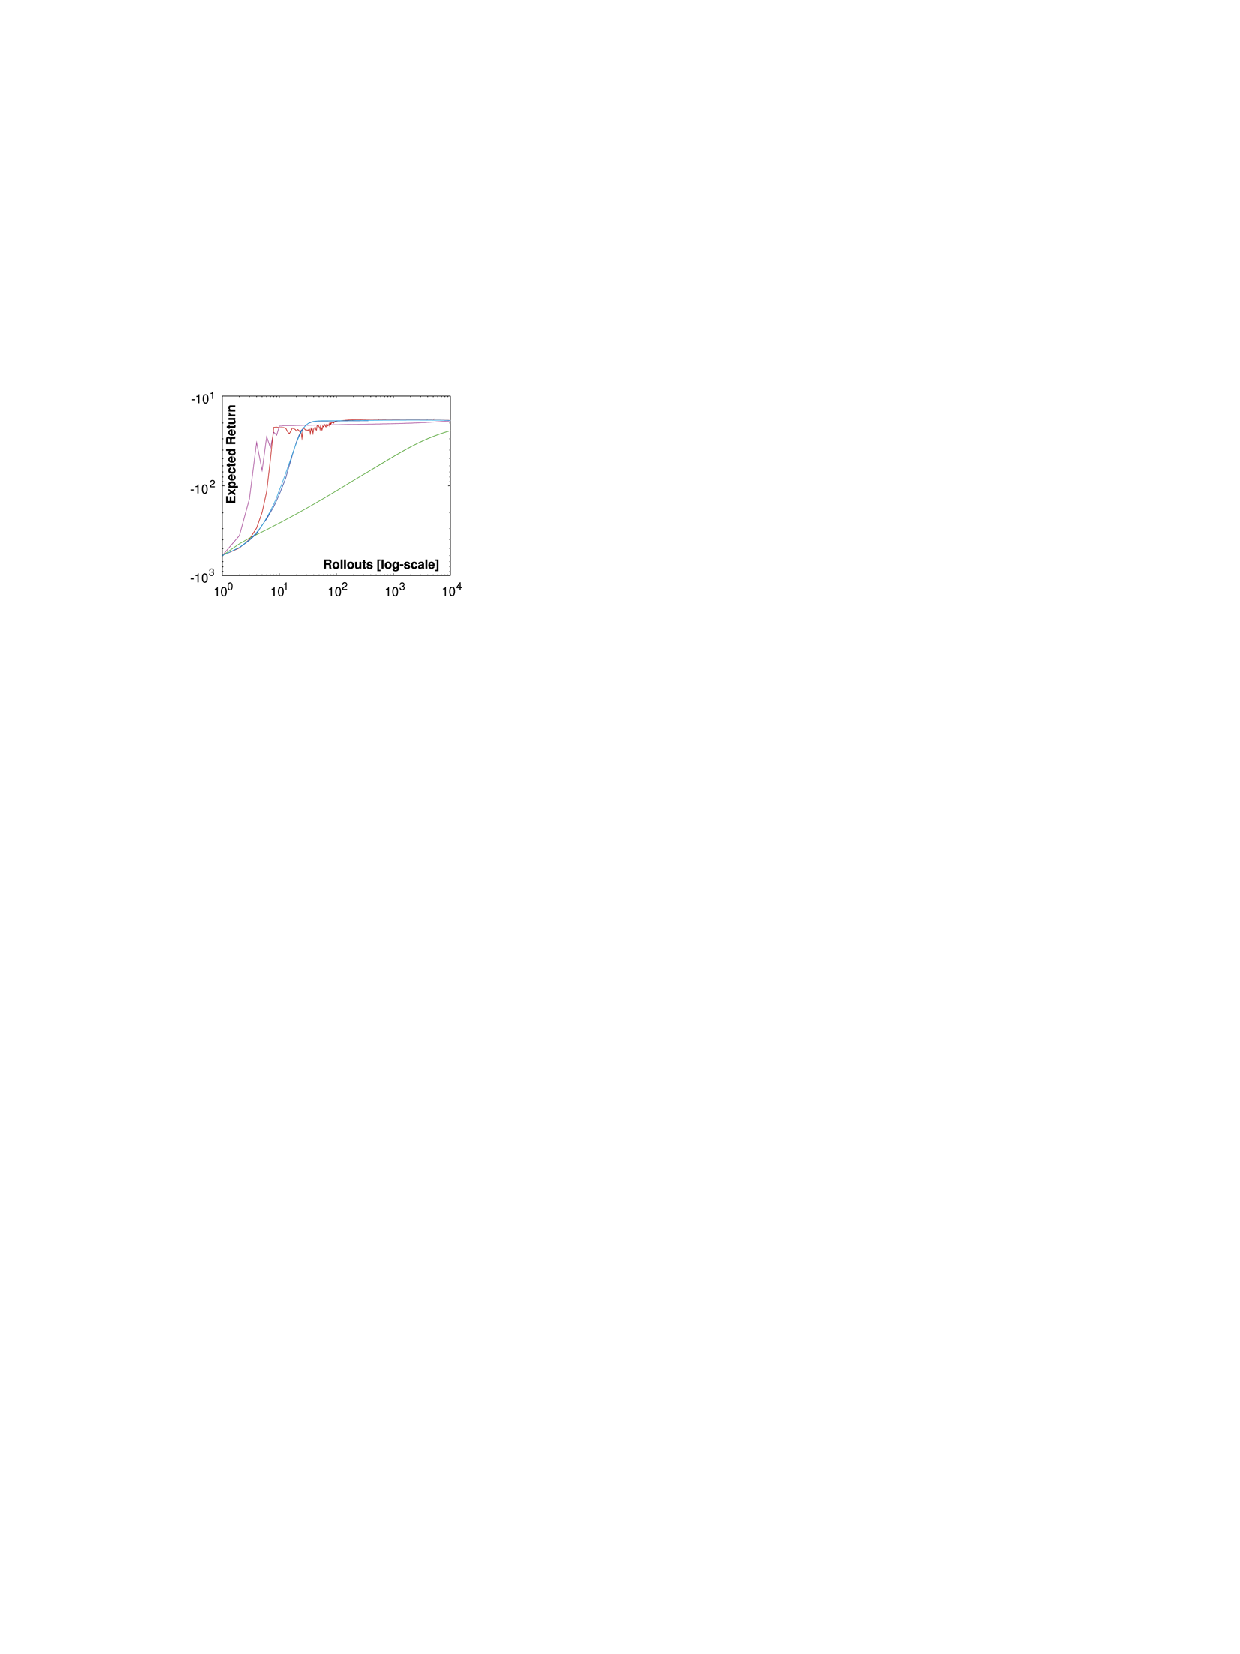
\includegraphics[width=0.4\textwidth]{Figures/NAC-minimum-motor-command.pdf}
\hfill
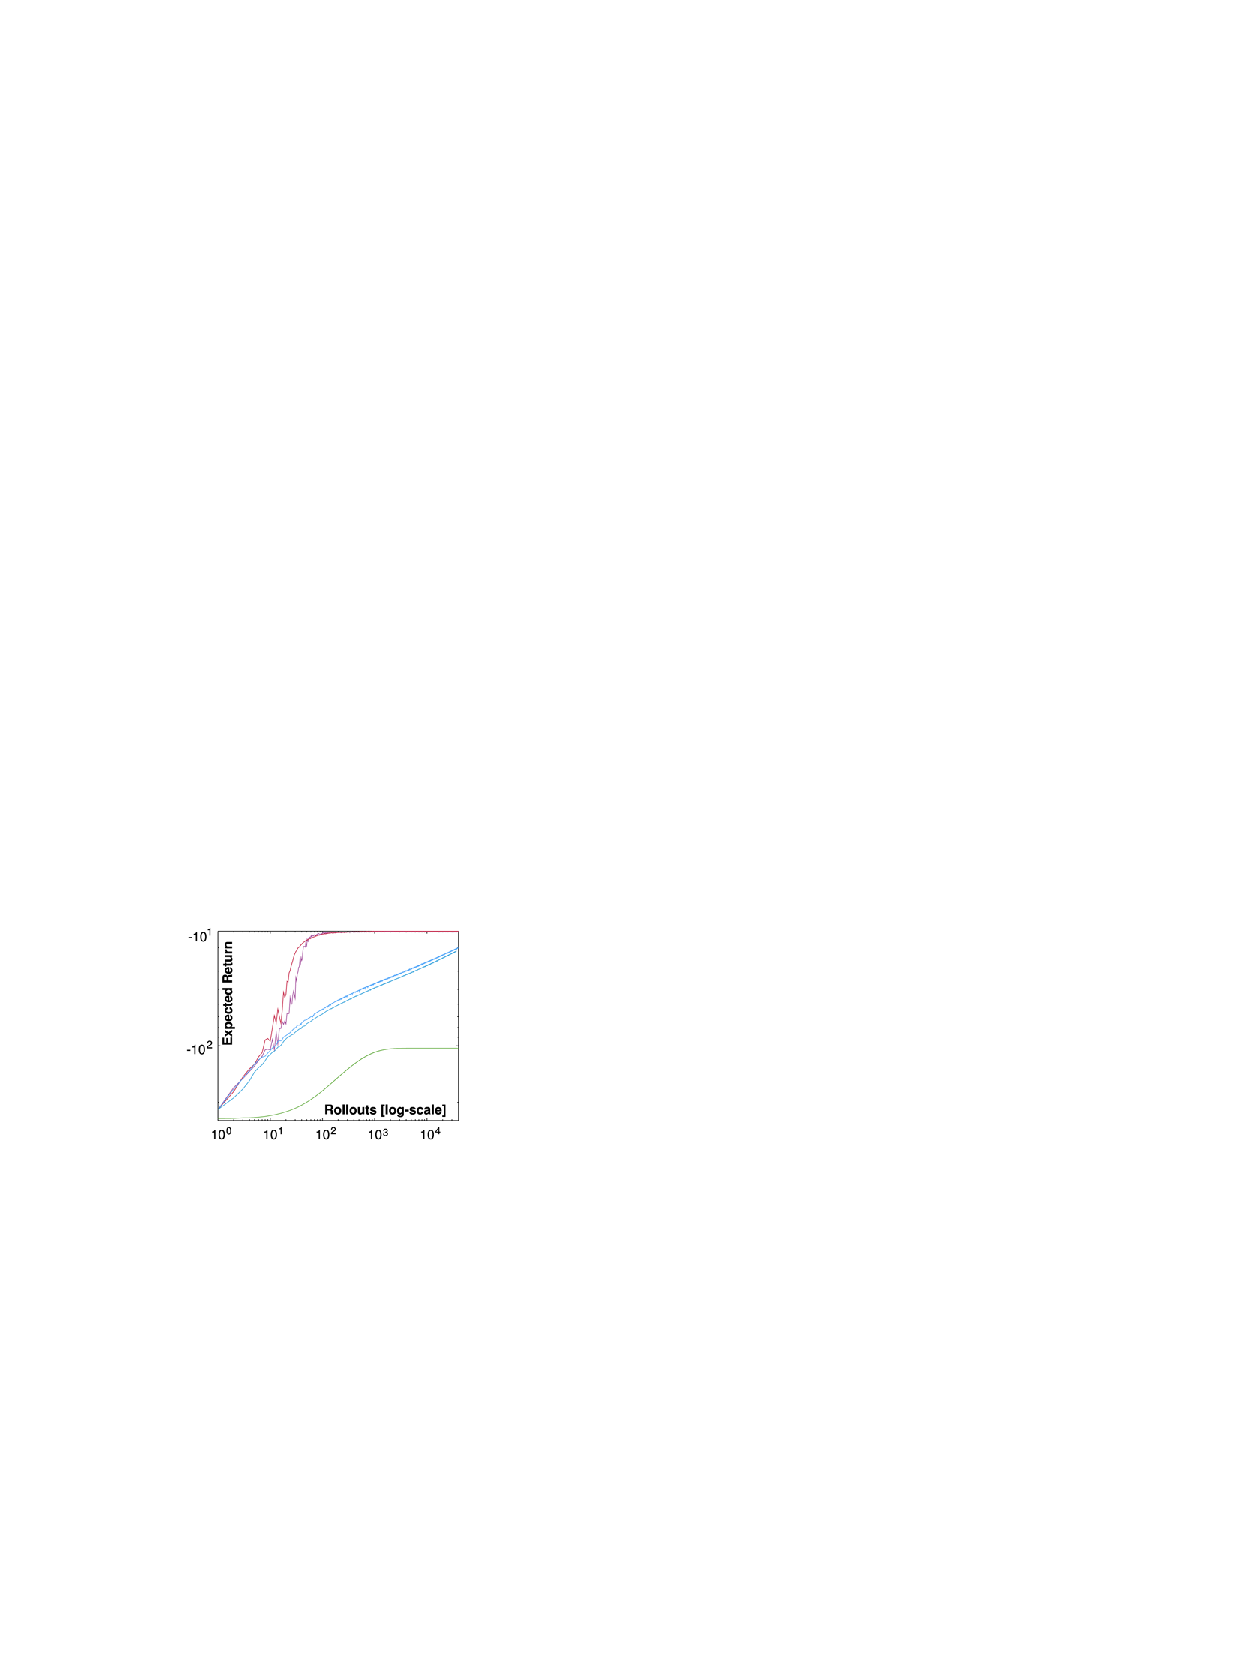
\includegraphics[width=0.4\textwidth]{Figures/NAC-passing-through-a-point.pdf}

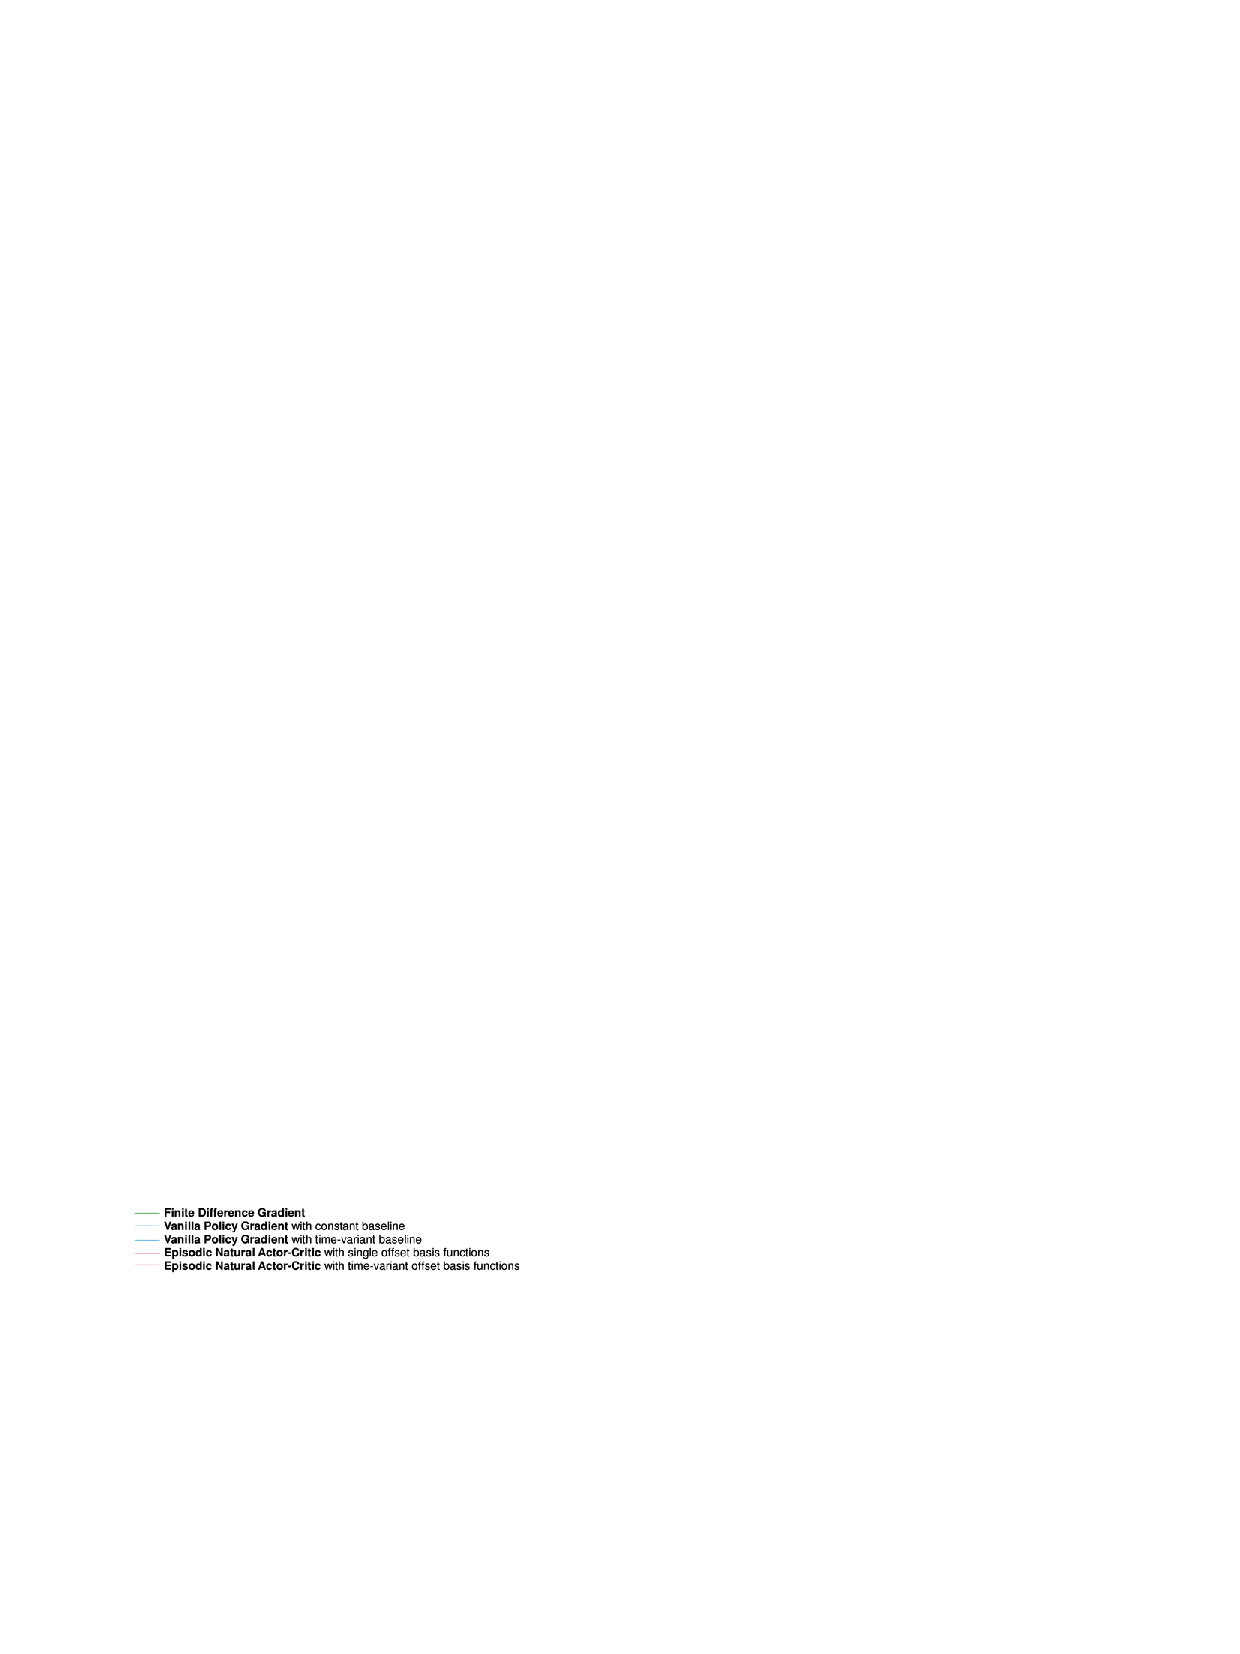
\includegraphics[width=0.4\textwidth]{Figures/NAC-legend.pdf}


Performance on problems (a) minimum motor command learning and (b) passing through a point.
\ec
\hfill \small Source: \citep{PeScha08:NN}
\note{
\bin
\item Dynamics: point mass control
\item Controller: ``motor primitives'' (a dynamical system with tuneable parameters, + a simple tracking controller (e.g. a PD controller), the motor primitives have some randomization in them
\item Perfectly observed state
\item Reward as per task
\item The point is that NAC is doing much better
\item (This NAC is somewhat strange, since then they can do even better.)
\ei
}
}


\animframen{Learning motor primitives with NAC}
{
\bc
\includegraphics<+->[width=\textwidth]{Figures/NAC-motorprimitive-learning.pdf}
\ec
\hfill \small Source: \citep{PeScha08:NN}
\note{
\bin
\item Application: learning to hit a baseball with an anthropomorphic robot arm (Sarcos Master Arm)
\item The task of the robot is to hit a (soft) baseball placed on a T-stick such that it flies as far as possible � this game is also known as T- Ball and is used in the US to teach children how to hit a baseball. 
\item The state of the robot is given by its joint angles and velocities while the actions are the joint accelerations. 
\item A given inverse dynamics controller is used to obtain motor torques from these kinematic variables. 
\item The ball position and velocity are observed through a color vision system (Newton Labs, MA) at 60 Hz video frequency.
\item The seven degrees of freedom of the robot are redundant during the hitting movement!
\item Reward: how the ball goes (terminal reward), minus the acceleration of the joints squared
\ei
}
}




\if0
\paragraph{Compatible function approximation}
Assume that a linear-in-the-parameters function approximation is used to estimate $\hQ_t$, but choose the feature-extraction function to be the score function underlying the policy class:
 \beq
 \label{eq:compatibleQ}
% \nabla_\theta Q_\theta = \nabla_\aparam \log \pi_\aparam
Q_\theta(\st,\action) = \theta\ttop \scorefun_\aparam(\st,\action), \qquad (\st,\action)\in \SA.
 \eeq
This choice of the function approximation method is called {\em compatible} with the policy parameterization.
Note that the basis functions depend on $\aparam$ (as $\aparam=\aparam_t$ changes, $\scorefun_\aparam$ will also change).
%(i.e., $Q_\theta = \theta\ttop \nabla_\aparam \log \pi_\aparam + V$ for some fixed function $V$).
What is a suitable value of $\theta$ for a fixed value $\aparam_t$?
Substituting  $Q_\theta$ for $\hQ_t$ in
 \eqref{eq:comp}, we get
\[
\EE{  \scorefun_{\aparam_t}(\St_t,\Action_t) \scorefun_{\aparam_t}(\St_t,\Action_t)\ttop }
\theta
=
 \EE{ Q^{\pi_{\aparam_t}}(\St_t,\Action_t)  \scorefun_{\aparam_t}(\St_t,\Action_t) }.
\]
Define $F_ \aparam = \EE{  \scorefun_{\aparam}(\St,\Action) \scorefun_{\aparam}(\St,\Action)\ttop }$,
$g_ \aparam = \EE{ Q^{\pi_{\aparam}}(\St,\Action)  \scorefun_{\aparam}(\St,\Action) }$
and
let
$\theta_*(\aparam)$ be the solution to the linear system of equations
\[
F_ \aparam \,\theta = g_\aparam.
\]
When this equation holds, $Q_{\theta_*(\aparam_t)}$ satisfies~\eqref{eq:comp}.
Notice that $\theta_*(\aparam)$ is the parameter that minimizes the mean-squared error
 \[
 \EE{ (Q_\theta(\St,\Action)-Q^{\pi_\aparam}(\St,\Action))^2}.
 \]
\fi

\section{Bibliography}
\begin{frame}[allowframebreaks=1]
  \frametitle{For Further Reading}
%  \begin{multicols}{2}
  \scriptsize\tiny
\def\newblock{\hskip .11em plus .33em minus .07em}
\bibliography{allbib,shortconfs}
%  \end{multicols}
\emptynote
\end{frame}

\begin{frame}
\bc
\LARGE DONE!
\ec
\end{frame}

\end{document}


% Doc: http://sourceforge.net/apps/mediawiki/skim-app/index.php?title=Tips_and_Tricks

% SKIM!! You need to open up the PDF of your presentation, as well as a second PDF of accompanying notes as the 'Synchronized Notes Document', containing exactly the same number of pages as the presentation. Then, in the presentation PDF, go to 'View' > 'Presentation Options', and in the dropdown for 'Synchronized Notes Document' you will see as an option the filename of the other PDF containing the notes for the presentation. Select that, then make sure you have the window of the presentation PDF on the 'public' monitor (eg a projector, as you would usually do) and the window of the notes document on your private monitor, such as your own laptop. Then simply put the PDF in presentation mode, and the notes PDF will scroll along as you change pages on the presentations PDF. 